\documentclass[10pt,a4paper]{article}
\usepackage{fontspec,xeCJK}
\setmainfont{Times New Roman}
\setCJKmainfont[AutoFakeBold=2,AutoFakeSlant=.2]{SimSun}
\setCJKmonofont{SimSun}
\usepackage[margin=20mm,top=22mm,bottom=22mm]{geometry}
\usepackage{paracol,graphicx,hyperref,xurl,fancyhdr,needspace,xcolor}
\hypersetup{unicode=true,hidelinks}\urlstyle{same}
\setlength{\columnsep}{8mm}\setlength{\parindent}{0pt}\setlength{\parskip}{5pt}
\setlength{\emergencystretch}{3em}\tolerance=2000
\widowpenalty=5000\clubpenalty=5000
\pagestyle{fancy}\fancyhf{}\fancyhead[L]{\small Candea and Heywood · Antiformalism}\fancyfoot[C]{\thepage}\setlength{\headheight}{14pt}
\begin{document}

{\Large\bfseries What Was Antiformalism, and What Comes Next? On Coherence, Corrigibility and Collaboration\par}\medskip

Matei Candea (Social Anthropology, Cambridge University, UK) and Paolo Heywood (Anthropology, Durham University, UK). Corresponding author: Paolo Heywood; paolo.heywood@durham.ac.uk. Comparative Studies in Society and History (2026), 1–27.\par
Reading edition based on the publisher HTML. Page labels refer to paragraph starting pages in the original 27-page PDF. The original table, five notes, all 123 references and HTML emphasis are retained. Original authors © 2026. CC BY 4.0. DOI separators have been added to the HTML references.\par
\url{https://doi.org/10.1017/S0010417526100589}\par
\url{https://creativecommons.org/licenses/by/4.0/}\par
Keywords: formalism; antiformalism; anthropological theory; structure; comparison; history of anthropology; emergence\par\bigskip
\Needspace{5\baselineskip}\section*{Abstract}
{\scriptsize\color{gray} [p. 1]}\ For several decades, social and cultural anthropology has been enmeshed in an antiformalist mood—a shared sensibility that valorizes disruption, emergence, and complexity over stability and pattern; celebrates flexible concepts resistant to systematization; and treats theoretical frameworks with suspicion. Initially revolutionary, this antiformalism has long since become mainstream, settling into recognizable conventions. This article traces antiformalism’s manifestations across diverse theoretical moments, from post-structuralism and practice theory through material and ontological turns, showing how form nevertheless persisted—often disavowed but relied upon—within ostensibly antiformalist approaches. We argue that the alternation between formalism and antiformalism constitutes something like the beating theoretical heart of anthropology, operating both at the macro level of half-century disciplinary shifts and at the microlevel of individual arguments where formal and anti-formal moves remain necessarily interwoven. Against this background, we detect an emergent tonal shift: a rising enthusiasm for form manifest in renewed attention to social and cultural regularities as puzzles worthy of explanation, and in a different valuation of conceptual work that emphasizes robustness, sharp edges, and shareability. We map this new formalist sensibility and identify its characteristic epistemic virtues—coherence, corrigibility, and collaboration—which distinguish it from both earlier structuralisms and recent antiformalist approaches, positioning anthropology as a diverse yet collective comparative endeavor.\par
{\scriptsize\color{gray} [p. 1]}\ \textit{“Each city receives its form from the desert it opposes.”}\par
{\scriptsize\color{gray} [p. 1]}\ \textit{Italo Calvino}\par
\Needspace{5\baselineskip}\section*{Introduction}
{\scriptsize\color{gray} [p. 1]}\ In her 1984 retrospective of “Theory in Anthropology since the Sixties,” Sherry Ortner began by noting that the discipline of the time appeared to be “a thing of shreds and patches, of individuals and small coteries pursuing disjunctive investigations and talking mainly to themselves” (Ortner 1984: 126). Famously, however, she went on to argue that such liminality was really “the breeding ground for a new and perhaps better order,” one focused on the “key symbol” of “practice” (ibid: 127).\par
{\scriptsize\color{gray} [p. 2]}\ In this piece we take a similarly retrospective approach to an anthropology that today too seems fragmented and anxious about its past, direction, and purpose (e.g., Bunzl 2008; Jobson 2020; Ortner 2015; Robbins 2013a; Sanchez 2023).\textsuperscript{1} Yet we feel, as Ortner did, that this liminality is the breeding ground for the emergence of a new pattern. This article aims to discern and sharpen the contours of a distinctive tonal shift in contemporary anthropology—not toward practice, now, but toward “form.”\par{\small 1. Whilst we refer to “anthropology” throughout this piece, we of course have socio-cultural anthropology in mind. Linguistic anthropology had a slightly different relationship to form throughout this period, to which we refer below. We leave to others the possibility of asking comparable questions of contemporary archaeology, or biological anthropology.\par}
{\scriptsize\color{gray} [p. 2]}\ For some decades now, social and cultural anthropology has been deeply enmeshed in an antiformalist mood or style, a shared sensibility about what counts as good anthropological work that cuts across the most diverse conceptual schools and thematic or regional subfields. This antiformalism is manifested in a broad set of contemporary expectations and preferences: 1) the valorization of accounts that emphasize disruption, emergence, and complexity at the expense of those that might be concerned with stability and reproduction of clear patterns; 2) the evaluation of theoretical frameworks based on their flexibility and resistance to systematization, at the expense of an emphasis on analytical precision or explanatory power (indeed, in some cases the very idea of explanatory “power,” like any other power, is held in suspicion—Latour 2005; cf. Heywood and Candea 2023); 3) the celebration of forms of writing that emphasize their own incompleteness and indeterminacy; 4) the related insistence that, because reality/practice/power exceeds or is messier than theoretical frameworks or analytical categories that seek to account for it, one ought to mistrust or discard such frameworks or categories; 5) a general intuition that form is inherently oppressive while formlessness is inherently liberating—epistemically, politically, and ethically.\par
{\scriptsize\color{gray} [p. 2]}\ Initially marginal and even revolutionary, such kinds of writerly and conceptual disruption have long since settled into a recognizable, mainstream genre (form) of their own, complete with conventions and tropes—George Marcus, always an astute observer of changing disciplinary aesthetics, once characterized this as a shift from the “experimental” to the “baroque” (2007). But this antiformalist aesthetic is not the exclusive appanage of the “writing culture” moment—nor indeed was “writing culture” itself exclusively antiformalist. The mood we have in mind is much broader. Indeed, the symbol of “practice” Ortner heralded, while it certainly displayed some formalist tendencies, also partook of this antiformalist aesthetic, with its commitment to dissolving strict divisions between structure and agency, history and stability, economics, politics, and culture. Nor is antiformalism merely a child of the eighties. Antiformalist intuitions also characterize some of the antecedents of “practice” Ortner describes (such as Geertzian symbolic anthropology) and stretch well into recent decades, far beyond the period of time in which the theoretical revolutions of the 1980s seemed fresh and novel.\par
{\scriptsize\color{gray} [p. 3]}\ Both of us, like most anthropologists of our generation and since, were raised in this antiformalist mood, and there is much that we still admire and share about its enthusiasms. The very notion of anthropological theory as in part a matter of moods, intuitions, and aesthetics is a clear example in this very paper. Nor is it a matter of dispute that the rise of antiformalism in the 1970s and 1980s coincided with a massive and deeply generative opening up of the discipline to new conceptual, thematic, and political possibilities. However, antiformalism’s successes mean it is now hard to think of it as marginal or revolutionary in the way it was at its beginnings.\par
{\scriptsize\color{gray} [p. 3]}\ Against the background of this pervasive and longstanding antiformalism we detect an emergent tonal shift, a broad and multi-polar convergence toward the sense that there might be more to form than we have been accustomed to think. Scholars of different generations and theoretical persuasions—including some whose own previous work bore marks of antiformalist enthusiasm—are rediscovering the beauty and utility of forms. Looking backward through this lens, we may find that formalism was already there, lying quietly below the noise and fury of grand disciplinary visions, holding anthropological arguments and comparisons together almost despite themselves, and waiting to be picked up and burnished to a brighter shine.\par
{\scriptsize\color{gray} [p. 3]}\ The return to form we explore in this paper combines two main strands. The first is an attention to the regularities of the world as something inherently interesting, puzzling, and worthy of explanation. The second is a different way of valuing conceptual and analytical apparatuses and devices, with an eye to robustness even at the cost of flexibility, and a vision of concepts as tools that can be shared with and taken up by others, hacked, patched, and put to other uses. Together these two aspects of the tonal shift to formalism outline a hopeful horizon for anthropology as a diverse, decentralized, yet still collective comparative endeavor.\par
{\scriptsize\color{gray} [p. 3]}\ The current regain of interest in form is not predicated on a particular ontological claim about the nature of social regularity. Anthropologists interested in form today are not reintroducing discredited assumptions about unchanging essences, bounded cultures, or fully functional social organisms. The regularities they attend to can be small, like a device, a technique, a social role, a scientific model (Helmreich 2014), or an example (Højer and Bandak 2015). They can be temporally shifting, like trends, agreements, styles of political presentation or humor, or even real estate speculation (Boyer 2013; Boyer and Yurchak 2010; Yurchak 2008; Humphrey 2020). They can be big, thin, and precise, like payment infrastructures (Maurer 2012), or big, loose, and unbounded, like the nevertheless palpable way in which cultures (Robbins 2007), formations (Asad 2003), scales (Summerson Carr and Lempert 2016; Lempert 2025), grammars (Kelty 2016), and semiotic ideologies (Keane 2018) shape contexts of intelligibility. Or like “modes” (Degani 2024), to which we return below, they can be a combination of all those things.\par
{\scriptsize\color{gray} [p. 3]}\ When we write of “form” in this article, we are indexing this wide range of worldly regularities, as well as the more obviously formal regularities of anthropological writing and concept-work itself.\textsuperscript{2} In the final part of the article, we focus in on the latter. In order to underscore the fact that conceptual formalism can itself take many forms, we distinguish two different types of conceptual formalism that have been on the rise in recent anthropology: the articulation of structured, systematic contrasts on the one hand, and the building of open-ended empirical lists on the other. Neither of these neo-formalist analytical heuristics is reducible to earlier anthropological concerns with “structure” and “system,” any more than the renewed concern with recognizing patterns in the world can be reduced to an avatar of earlier anthropological positivism. Perhaps the most important take-home point here is that, as we write below, the current anthropological return to form does not answer the question of regularity—it poses it. In closing, we explore what we feel are three distinctive epistemic virtues that are self-consciously associated with the new formalist aesthetic: coherence, corrigibility, and collaboration.\par{\small 2. There are other ways to refer to this general problematic (modes, cultural categories, scales, etc.). We have selected form, partly because it points with particular insistence to this double regularity in the world and in the account.\par}
{\scriptsize\color{gray} [p. 4]}\ In sum, this article is both descriptive and programmatic: it outlines the current tonal shift toward an embrace of form in anthropology, situates it in relation to a now waning antiformalism, analyzes its conceptual underpinnings and effects, and wishes it well.\par
\Needspace{5\baselineskip}\section*{Enthusiastic Reversals and Underlying Stabilities}
{\scriptsize\color{gray} [p. 4]}\ This is not the first time in the history of anthropology that form has emerged as a key trope and hope. If structure was stale by the 1970s, in the early-to-mid-twentieth century, tracing social or conceptual forms and structures was for many the exciting alternative to the perceived limitations of earlier ethnographic or ethnological particularism. But that turn-of-the-twentieth-century anthropological particularism itself had been the exciting alternative to the teleological formalism of nineteenth-century evolutionist comparatism (for a more nuanced account of this set of reversals, see Strathern 1987, Candea 2019). The formalist-antiformalist contrast we describe, in other words, is one that has manifested itself in a range of avatars, but outlasted any single pair of them.\par
{\scriptsize\color{gray} [p. 4]}\ Such shifts in enthusiasms are not merely intellectual fads. Antiformalism has been a political as much as an epistemic persuasion. But the political affordances of antiformalism, like the politics of formalism, are various. If antiformalism in the 1960s and 1970s was self-consciously entwined with progressive attacks on the “old order,” recent political transformations have seen the rise of a triumphant antiformalism of the most reactionary kind—and not for the first time, as historians and ethnographers of fascism can attest (Heywood 2023; 2024). Conversely, formalism may stand for the politics of the “radical centre,” or \textit{ancien régime} quietism (“structures don’t take to the streets” ran a French May 68 slogan); but formalism also informed revolutionary Bolshevism and can animate radical prefigurative politics (Krøijer 2015), a principled resistance to neoliberal disruption (Du Gay 2000) or to colonialism (Limbert 2025).\par
{\scriptsize\color{gray} [p. 4]}\ The alternation of formalism and antiformalism is something like the beating theoretical heart of the discipline. This is true not only on the macroscale, as moments of formalist and antiformalist enthusiasm alternate every half-century or so, but also on the microscale, as formal and anti-formal moves interweave in every anthropological account. How can both of these things be true at the same time? To see this, we must distinguish the microphysics of anthropological argument from the broader aesthetic currents that inform disciplinary enthusiasms. At the level of individual anthropological arguments and texts, formalism and antiformalism are necessarily interwoven, as concepts are defined, critiqued, and unmade, moments and vignettes held up as sui generis and then rendered partly fungible through comparison, substantive particulars brought to bear to challenge broader generalities, and in turn held up as characteristic of broader forms. Conceptually, anthropologists are forever making theoretical patterns and breaking them. Empirically, every account of a social, cultural, or material regularity implies its obverse—exception, hybridity, and irregularity—and vice versa. At this basic level, form and formlessness are simply the warp and weft of anthropology.\par
{\scriptsize\color{gray} [p. 5]}\ This interplay of formal and anti-formal moves at the microlevel also often manifests itself methodologically, as for instance where multi-sited ethnography resists the imaginary of the bounded field site yet relies on implicit wholes to operationalize this resistance (Candea 2007), or when “ethnographic refusal” operates as a formal device of strategic exclusion in order to resist attempts at formal description. The microlevel interplay between the making and unmaking of forms operates as much in how we conduct research as in how we theorize it. Indeed, beyond these particular examples, it is evident in the granular fixes and adaptations that any fieldwork experience must involve.\par
{\scriptsize\color{gray} [p. 5]}\ But form and its negation do not register in the same way when anthropologists think, more broadly, about what is valuable, new, and exciting in their discipline. Formalism and antiformalism, on a broader scale, denote a feeling about what is valuable and worthwhile in our various theoretical apparatuses and empirical descriptions. They are sensibilities, aesthetics; they delineate what is exciting and what is just necessary, what is new and what is old, which problems and concerns are natural and obvious, and which feel forced and artificial by contrast. Our argument therefore is not that form has been absent from anthropology over the past fifty years—that would be nonsense—but rather that form has often been treated with suspicion or disinterest. Over the past half-century or so, anthropologists have of course acknowledged the existence of socio-cultural regularities, but it is striking how often they have done so while being primarily excited by and attentive to the exceptions to such formal patterns—teeming multiplicity, liminality, hybridity, assemblage, transformation, and contingency. Over the same period, conceptual distinctions, dichotomies, and other formal-sounding analytics have also been generated—indeed, it is a paradox of antiformalism that it churns through conceptual forms at great speed. But these conceptual formalisms have tended to be presented or experienced as a necessary evil along the path to a more faithful, less formally constrained account of the vital multiplicity of the world.\par
{\scriptsize\color{gray} [p. 5]}\ To put it otherwise, the major mood of the past fifty years was antiformalist, and yet a minor formalism persisted within anthropological arguments and approaches. Over the next two sections we trace this minor, buried, or encompassed formalism, before turning to the current reversal of polarities that is bringing form to the foreground. We welcome and share this rising enthusiasm for form, even as we recognize the debt it owes to the antiformalist enthusiasms that seem now to be on the wane. The point of this article, therefore, is not to advocate abandoning attention to contingency, complexity, and other associated antiformalist objects, but to make the case for form’s renewed value. Our aim is diagnostic in attempting to identify a shift in disciplinary sensibilities, but it is also programmatic in welcoming this shift and articulating some aspects of its promise. Indeed, the very attempt at comparative assessment we aim to undertake here is arguably itself a characteristically formalist move, as is the formalist/antiformalist distinction with which we operate. Whether that particular distinction and our particular comparison persuades readers or not, we hope to make the case for a renewed attention to distinctions and comparisons more generally.\par
\Needspace{5\baselineskip}\section*{The Form in Antiformalism 1: Post-structuralism, Practice Theory, and Material Turns}
{\scriptsize\color{gray} [p. 6]}\ Giving form to antiformalism means trying to see a thread that is woven through the “thing of shreds and patches” that anthropology has been for some time. In previous and separate work we have both sought to trace how this thread manifests across diverse theoretical moments: one of us has analyzed the ways in which both 1980s post-structuralism and turn-of-the-millennium materialist approaches in anthropology constituted “twin pincers” of antiformalism (Candea 2025); the other has shown how Wittgenstein’s influence on anthropology, from Geertz through to Veena Das and other contemporary work, involved a progressive collapse of contextual form (Heywood 2026).\par
{\scriptsize\color{gray} [p. 6]}\ What emerges from these analyses is not the absence of form or formal elements from recent anthropological work, but a sense of their widespread subordination to antiformalist priorities.\par
{\scriptsize\color{gray} [p. 6]}\ It is not difficult to point to the antiformalist elements of post-structuralism: heralded by the crisis of representation, anthropological post-structuralism positioned form—whether analytical or empirical—as an instrument of power to be resisted. Antiformalism was thus simultaneously an epistemic and a political project (Candea 2025: 4). Postmodern anthropologists shared an “orientation toward cultural order,” to quote James Clifford (1981: 539), “[f]rom [whose] disenchanted viewpoint stable orders of collective meaning appear to be constructed, artificial, and indeed often ideological or repressive. The sort of normality or common sense that can amass empires in its fits of absentmindedness or wander routinely into world wars is seen as a contested reality, to be subverted, parodied, and transgressed.”\par
{\scriptsize\color{gray} [p. 6]}\ This sensibility filtered through in their attitude to conceptual forms also. Postmodern anthropologists shared with theorists from other disciplines an epistemico-political commitment to de-formalizing analysis, “to recall what our structures and systems produce and suppress as they impose order in the world and to affirm [formlessness] as capable of breaking or deforming those structures and systems from within their limits” (Gandolfo 2013).\par
{\scriptsize\color{gray} [p. 6]}\ This deep suspicion of conceptual systems and structures as inherently linked to historical and political violence is still very much with us. It is echoed particularly starkly, for instance, in contemporary work on “ethnographic refusal.” Thus, Audra Simpson draws a direct link between the colonial and imperial project and anthropological concerns with “sorting, ordering, and ranking”: “[T]hese colonial encounters were and still are a mess of disorder, of so-called transformation, of dispossession of people from land and culture. The easy answers for the emergent field were the ethnological grid; the kinship chart; the orderly, predictable clan unit” (2016).\par
{\scriptsize\color{gray} [p. 6]}\ And yet, for all their explicit suspicion of form, there was also a powerful formalist aesthetic at play in some of the key contributions to the “writing culture” turn, as there is to the very different intellectual genre of “ethnographic refusal.”\par
{\scriptsize\color{gray} [p. 6]}\ The attention to anthropological texts \textit{as texts}, and a concern with the aesthetics of knowledge production, led writing culture anthropologists to dissect, categorize, and experiment with prose in deeply formalist ways. Formal devices and concerns were central to the writing culture moment, and indeed it is in their wake that our own arguments about disciplinary “aesthetics” and “sensibilities” take shape.\par
{\scriptsize\color{gray} [p. 7]}\ The same forebears also inform the conceptual, empirical, and literary use of exclusions, cuts, and redactions that mark ethnographic refusal as a “methodological form” (McGranahan 2016). And yet, it is the critique of form, rather than the formalist intuitions of the crisis of representation—or more recently of “ethnographic refusal”—which has been most marking and remarked upon.\par
{\scriptsize\color{gray} [p. 7]}\ As Ortner points out in her discussions of “practice,” this kind of post-structuralist antiformalism did not emerge \textit{ex nihilo} . Just as Geertzian anthropology is central to Ortner’s genealogy of “practice” (1984: 130), so it is also an important step in the story we tell here. Geertz drew heavily on the later Wittgenstein to articulate a vision of anthropology that was significantly influenced by the latter’s antiformalism (Heywood 2026). The vision in question is neatly condensed by Geertz’s student Richard Shweder in characterizing Geertz as “Wittgenstein’s anthropological reincarnation”: “For in some of Wittgenstein’s writings, Geertz apparently discovered a philosophy—one opposed to big-systems thinking and ideas about universally fixed essences—that suited his temperamental disinclination to be pinned down…. In accord with Wittgenstein, Geertz saw reality as an almost unthinkably complex continuum of overlapping likeness and differences that it was a bad job or a kind of violence to try filing into neat boxes…. ‘I don’t do systems,’ he would say” (Shweder 2007: 201–2; cf Heywood 2026).\par
{\scriptsize\color{gray} [p. 7]}\ Yet despite that last claim, Geertz’s training under Talcott Parsons in systems theory left clear traces in his concept of “cultural systems,” like religion, that maintain coherent formal properties across different instantiations. His textualism, like that of \textit{Writing Culture}, implied systematic interpretive frameworks with discernible patterns. And as critics noted, his deployment of the culture concept and his “thick description” could, despite his desire to avoid reductive formalism, lead to essentializing accounts that rendered “the Balinese” into what appeared to be a coherent and bounded unit.\par
{\scriptsize\color{gray} [p. 7]}\ Or take “practice”: practice theory shared with \textit{Writing Culture} anthropology many of Geertz’s (and Wittgenstein’s—Bourdieu was a devotee) antiformalist preferences. Yet Bourdieu is an excellent example of the point that antiformalist enthusiasms can thrive on a formalist base. Bourdieu’s aims were in many ways quintessentially antiformalist: to dissolve structure into process, stability into change, rules into strategies, and analytical binaries into the polysemy of practice. This understanding of practice is what is most traveled in anthropological usage.\par
{\scriptsize\color{gray} [p. 7]}\ Yet Bourdieu himself produced some of the most eminently formalist work of his generation: detailed analyses of fields, doxa, and habitus, alongside precise taxonomies of aesthetic judgment and cultural capital. His method was built on formal “distinctions,” not to mention quantitative analysis and systematic comparison. The apparent paradox of “structuring structures” is at least as much a formalist attempt to synthesize pattern with change as it is an antiformalist dissolution of the boundary between the two (1977).\par
{\scriptsize\color{gray} [p. 7]}\ The uptake of Bourdieu’s work illustrates this well. Marshall Sahlins retained many of his formalist commitments even as he turned from structuralism to practice theory—and this was often held against him. One of us vividly recalls having Sahlins’ theory of history disparaged by an undergraduate supervisor as “structuralism with an outboard motor.” As in this example, by the late 1990s, the claim that practice theory was, in some way, residually formalist or “crypto-formalist” was often articulated as a critique.\par
{\scriptsize\color{gray} [p. 8]}\ Foucault’s work, similarly, has left a deep mark in anthropology through an understanding of power as so dispersed, relational, and unspecifiable that it is ubiquitous. Yet Foucault’s concepts of episteme, archive, and discourse imply rigorous analytical frameworks for understanding systems of power and knowledge \textit{as systems.} And his late work on ethics famously offered a detailed quadripartite schema for analyzing practices of self-cultivation. This more formalist Foucauldian legacy is exemplified in the work of scholars like Paul Rabinow, who deployed notions of form prominently in his \textit{French Modern} (1989, see also 1996). Other scholars in the same tradition often retained this attention to form in their work (see for instance Langlitz 2020; Rees 2018)—most notably perhaps James Faubion in his thorough and systematic explorations of Foucault’s analytic of ethics (2011). This formalist Foucauldian legacy stands out amongst—and illustrates by contrast—the far more common invocation of Foucault as the theorist of “power, power everywhere” (Sahlins 2002).\par
{\scriptsize\color{gray} [p. 8]}\ Antiformalism is even clearer in the influence of the other significant post-structuralist thinker with an anthropological legacy, Gilles Deleuze: “In emphasizing the powers and potentials of desire…the ways in which social fields ceaselessly leak and transform (power and knowledge notwithstanding), and the in-between, plastic, and ever-unfinished nature of \textit{a} life, Deleuze lends himself to inspiring ethnographic efforts to illuminate the dynamism of the everyday and the literality and singularity of human becomings.… ‘To write is certainly not to impose a form (of expression) on the matter of lived experience,’ says Deleuze. ‘Literature rather moves in the direction of the ill-formed or the incomplete’” (Deleuze 1997: 1, quoted in Biehl and Locke 2010: 318–20; italics in original).\par
{\scriptsize\color{gray} [p. 8]}\ Yet Deleuze too developed, with Guattari, elaborate taxonomies of social formations (bands and empires), typologies of semiotic regimes, and detailed mappings of “abstract machines.” Even his critique of “arborescent” thinking relies on a formal contrast between the tree and the rhizome.\par
{\scriptsize\color{gray} [p. 8]}\ The idea of “the matter of lived experience,” and the concrete particulars of “\textit{a} life” brings us to what we might think of as the second wave of anthropological antiformalism. The 1990s saw a clear turn away from “mere form” toward “what matters” (Candea 2025: 6). The material turn in many ways amplified rather than abandoned the antiformalism of post-structuralism. Matter was just as opposed to form as was textual antiformalist “play.” Yet materialist approaches also often contained sophisticated formal elements: approaches to embodiment developed systematic phenomenological frameworks for understanding experience; environmental anthropology has deployed ideas from ecology and systems theory; Actor-Network Theory offered precise protocols for mapping out associations between “actors” and “actants”; and the “ontological turn” was to some extent premised on the possibility of what Martin Holbraad calls “conceptual morphology” (2020).\par
{\scriptsize\color{gray} [p. 8]}\ Yet these systematic elements are often overshadowed by a distinctive kind of “two-step dance” (Heywood 2026). In the first step, a commitment to the “really real”—bodies, matter, objects, things—is characterized as the proper, overriding duty of anthropology. In the second step, this reality is revealed as one version or another of a “processual-relational haze” (Humphrey 2008: 358). Emily Martin’s pioneering \textit{Flexible Bodies} (1994), for example, attended to the concrete realities of health and immune systems, but it also resolved these realities into “configurations,” a term meant to refer to “a pattern or shape (\textit{more or less fuzzy}) that is simultaneously how we see the world and a result of how the social world is ordered” (ibid: 15; our italics). Actor-Network Theory refigured the meaning of reality by conjuring its networks as “flat ontologies,” undifferentiated by anything more substantial than the artifice of analysis (Latour 2005). And the ontological turn led to accounts that resembled each other in finding antiformalist processual becoming and non-dualist ontologies wherever they looked (Heywood 2012; Laidlaw and Heywood 2013; Candea 2016).\textsuperscript{3}\par{\small 3. We should note that attention to process need not be antiformalist, and that a range of recent scholarship (e.g., Fleming 2024; Hull 2012; Zuckerman 2020) attends to both processual dynamics and formal properties without seeing the two as necessarily opposed.\par}
{\scriptsize\color{gray} [p. 9]}\ More recently, even Brian Larkin’s compelling and persuasive call for studies of material infrastructure to attend to “form” in various ways nevertheless echoes in some ways the same underlying picture: “One of the most exciting sides of new materialism is its emphasis on emergence and the becoming of matter rather than its fixed ontology (Barad 2007; Coole and Frost 2010). I see the dynamics of encounter as formed through the constant evolution of objects in relation to discrete environments…the relationship between the material and the figural—particularly in the case of infrastructures—is reciprocal and entangled rather than causal and successive” (Larkin 2017: 197–98).\par
{\scriptsize\color{gray} [p. 9]}\ In sum, form has been with us throughout the many turns and twists of the past half-century of anthropological theorizing, but it has often, as here, been encompassed by emergence, and systematic analysis by relational entanglement.\par
\Needspace{5\baselineskip}\section*{The Form in Antiformalism 2: Concepts as Constraints}
{\scriptsize\color{gray} [p. 9]}\ Beyond identifiable “turns” such as those ontological, infrastructural, or (Deleuzian) affective, the dominant antiformalist thread is also identifiable in the kinds of “portable analytics” (Howe and Boyer 2015) that have defined the discipline for some time and that travel across a range of fields.\par
{\scriptsize\color{gray} [p. 9]}\ “Everyday life,” for example, or the use of “everyday” or “ordinary” as an adjectival marker before a particular phenomenon, has become a ubiquitous object in both anthropology and the wider social sciences, functioning thus as both a transcendent formal category and a marker of specificity (cf. Heywood 2023; 2024). The last three decades have witnessed an extraordinary expansion of the category across anthropology and beyond. One can find “everyday life” (or everyday violence, or everyday ethics, or everyday religion, or everyday politics, etc.) everywhere, and yet what one discovers in any given instance should be irreducibly specific, concrete, and particular. The result is a general concept that denies its own generality, producing what Marilyn Strathern identified in the 1990s as a flattening effect that erases form: writing of the comparable sociological notion of “family life,” she noted that “all the variability of family forms are thus flattened out in the assertion that everyone has some sort of family life” (1992: 145). Everyday life performs the same operation, gesturing simultaneously to (formless) generality and (formless) particularism.\par
{\scriptsize\color{gray} [p. 9]}\ Yet “everyday life” implies (formal) distinctions between the ordinary and the extraordinary, routine and event, background and foreground. It establishes formal hierarchies (the everyday as the foundational scale of interaction), and spatial boundaries (domestic versus public). Much of its analytical power derives from these properties.\par
{\scriptsize\color{gray} [p. 10]}\ In somewhat similar fashion, the strength of “neoliberalism” as an analytic is sometimes said to reside precisely in its capacity to contain its own negations (Muehlebach 2010). Whilst there is a flavor of the “power, power everywhere” functionalism that Marshall Sahlins diagnosed in 1980s Foucauldian anthropology in this capaciousness (Sahlins 2002), it is also very much in line with a disciplinary aesthetic that privileges unbounded analytics as ways of coming to terms with an unbounded world (see also Degani 2022). And yet neoliberalism began its life as a classic categorical term distinguishing a specific historical moment and a particular political-economic dispensation, and those who use it do so with an at least residual attachment to this formalist legacy, even as they seek to bend the term to encompass new realities.\par
{\scriptsize\color{gray} [p. 10]}\ Other recent anthropological keywords, from “gens” to “assemblage,” exhibit similar characteristics: “gens” is a “capacious, flexible term that references our interest in the generative powers of capitalism and the inequalities these powers create” (Bear \textit{et al.} 2015; see also Sanchez 2024 for critique of this flexibility). “Assemblage,” exemplified in Anna Tsing’s discussions of Matsutake mushrooms, is a term used to denote “indeterminacy and the conditions of precarity, that is, life without the promise of stability…the uncontrolled lives of mushrooms are a gift—and a guide—when the controlled world we thought we had fails” (Tsing 2010: 2). Here again, formlessness and flexibility are valued even though the concepts are still, at least residually, intended to frame phenomena and guide interpretation.\par
{\scriptsize\color{gray} [p. 10]}\ The frequent insistence that concepts ought to be flexible, capacious, or vague might seem to undermine what concepts are supposed to do in the first place—frame, define, contain, and distinguish. However, this desire for flexibility relates to the intuition that limiting, systematizing, and framing are already pervasive, given, and in many respects unfortunate. This is a core intuition of antiformalism—that form is in fact everywhere in thought and therefore needs to be combated. This—dare we say residually structuralist—intuition guides an approach to concepts in which the problem of intellectual production is to loosen or fight against the ubiquitous power of form, in order to really do justice to the emergent unformed complexity of the world. Hiro Miyazaki has called this an “aesthetics of emergence,” in which, as anthropologists become concerned with their belatedness in regard to an emergent world, the “task becomes simply to trace or track the world as it emerges [and] knowledge itself is rendered emergent in order to mirror an emergent world” (2004: 138). Miyazaki traces this aesthetic to the 1980s, and yet this is a vision that dates back at least to Geertz and his Wittgensteinian conceit that “an accurate picture of a vague object does not consist of a clear picture but a vague one” (Geertz, Geertz, and Rosen 1979: 199; see also Heywood 2026). Conceptual form and systematicity are, to this view, the obvious starting point, the tools anthropologists are given to begin with, and these are too blunt, too strict, and limiting to really trace the emergent world. Concepts are a necessary enemy one needs to strain against.\par
{\scriptsize\color{gray} [p. 10]}\ Deleuze and Guattari’s description of their relationship to their own dualisms (such as the distinction between rhizome and root) is exemplary of the logic here—albeit unusual in its explicitness: “We invoke one dualism only in order to challenge another. We employ a dualism of models only in order to arrive at a process that challenges all models. Each time, mental correctives are necessary to undo the dualisms we had no wish to construct but through which we pass [to] arrive at the magic formula we all seek—PLURALISM = MONISM—via all the dualisms that are the enemy, an entirely necessary enemy, the furniture we are forever rearranging” (Deleuze and Guattari 1988: 20–21).\par
{\scriptsize\color{gray} [p. 11]}\ Using models—necessarily, unwillingly, and as if against one’s better judgment—while striving for the impossible horizon of a process that challenges all models: that is the essence of the antiformalist aesthetic of concept use.\par
{\scriptsize\color{gray} [p. 11]}\ Beyond the valorization of concepts for their flexibility rather than for their precision, this aesthetic manifests itself in several other ways, including but not limited to: 1) resistance to causal attribution or the idea of a corrigible account; 2) a preference for description over explanation (Heywood and Candea 2023); 3) the celebration of analytical open-endedness as an (or even \textit{the}) epistemic virtue; 4) emphases on the description of process, relation, emergence, and transformation over accounts of stasis, entities, or stability.\par
{\scriptsize\color{gray} [p. 11]}\ Our point, then, is not that the past half-century of anthropological theorizing has done without any reference to social, cultural, and analytical forms, or that it produced writing that was genuinely “formless.” Rather the point is that otherwise radically diverse arguments and theoretical movements have cast forms as the enemy, while nevertheless relying on them, sometimes in a more or less disavowed way. Formlessness was a horizon, and forms were necessary evils on the path toward it. Antiformalism, in its more self-conscious avatars, might be described as an ascetic striving away from forms experienced as necessary and ubiquitous. As in other ethical traditions, “it is in that dynamic tension between precept and practice that asceticism is really lived” (Laidlaw 1995: 7).\par
{\scriptsize\color{gray} [p. 11]}\ This antiformalist dependency on forms has multiple sources. Logically, oppositional concepts require one another for their definition, as Jonathan Culler notes when he describes the “strange result” of post-structuralism to be “that the vocabularies, procedures, and results of structuralist thinkers are preserved and celebrated but the frameworks of systematic projects are often bracketed or set aside” (Culler 2018: 93). This pattern extends beyond post-structuralism, through to antiformalist anthropology of a more recent vintage. Concepts like “practice,” “process,” “emergence,” “matter,” “flow,” and “becoming” gain their analytical power precisely through their opposition to “structure,” “stasis,” “form,” and “being,” but this oppositional definition makes them conceptually dependent on what they reject.\par
{\scriptsize\color{gray} [p. 11]}\ This dependence becomes particularly evident in substantive analytical work. To meaningfully discuss liminality, borders, migration, hybridity, and flows—characteristic concerns of antiformalist anthropology—one necessarily requires an underlying social morphology that defines what counts as center versus margin, inside versus outside, stable versus mobile, pure versus mixed. “Border crossing” becomes analytically interesting because it presupposes, at least to some extent, stable entities with definable boundaries that can be crossed. “Hybridity” depends, at least to some extent, on notions of distinct forms that can be mixed. “Migration” requires, at least to some extent, concepts of discrete places between which movement occurs (see Limbert 2025). Yet it is usually not the formal frameworks that would make such distinctions analytically explicit and defensible that hold our attention or interest, and indeed we often disavow them whilst nevertheless relying on them implicitly.\par
{\scriptsize\color{gray} [p. 11]}\ This dependent relationship extends also to basic practical and methodological considerations: ethnographic work celebrating multi-sitedness, emergence, flow, and indeterminacy still requires practical decisions about where to work, whom to interview, what to observe, how to organize findings, and, perhaps crucially, \textit{where to stop} (Candea 2007). These decisions implicitly invoke formal categories—communities, institutions, practices, events—even when the analysis explicitly rejects such formalism.\par
{\scriptsize\color{gray} [p. 12]}\ This general approach to analytical work as a struggle against form stems from a coherent albeit often implicit set of assumptions about the relationship between knowledge and the world. Knowledge is taken to be essentially and disappointingly formal, while the world is excitingly substantial and emergent. The key problem of knowledge production is to fight against the insufficient and always inadequate conceptual formalisms we have inherited in order to get ever closer to the generative formlessness of the world.\par
{\scriptsize\color{gray} [p. 12]}\ All of this means that any kind of antiformalism has a metaphysics, even when this metaphysics may be experienced as an anti-metaphysical stance (Heywood 2026). Because such claims about knowledge and the world are always framed as in opposition to metaphysics, to formalism, or to theory, they may not appear as such, but their effect may be just as constraining if not more so than earlier anthropological formalisms. More so, potentially, because such approaches may feel themselves precisely liberated from such formal constraints. The philosopher Tristan Garcia has pointed to a similar consequence of the modern obsession with antiformalist “intensity” in the work of thinkers like Nietzsche, Whitehead, and Deleuze: “An unheard of difficulty came to light as the concept of intensity was generalised throughout the arts and sciences of the twentieth century. Paradoxically, it seems that the absolute victory of intensity is also a sign that its defeat is drawing nigh. To make an entity absolute is also to annihilate it…[o]nce identified, intensities soon cease to be recognisably intense” (2018: 58).\par
{\scriptsize\color{gray} [p. 12]}\ What we have tried to suggest thus far, though, is that the formalism disavowed by much contemporary anthropology has a tendency to return in displaced form: theoretical frameworks that place great emphasis on rejecting systematicity develop their own implicit systems; approaches that celebrate methodological or rhetorical flexibility generate their own orthodoxies; concepts designed to resist formal specification acquire informal but nonetheless constraining conventions of usage. The trouble, as one of us wrote elsewhere, is that the power and effectiveness of antiformalist conceptual devices “comes from the continued relevance of what they negate. To generations of anthropologists whose training still relied on formal devices—kinship structures, modes of production, patterns of culture—‘the everyday,’ ‘gens,’ and ‘actor-networks’ were genuinely liberating. As they become the standard background of anthropological training, however, and the older forms they sought to unseat have receded into history, their ability to shed light on phenomena necessarily fades” (Candea 2025: 52–53).\par
\Needspace{5\baselineskip}\section*{Toward Form 1: Not Everything Is Shapeless}
{\scriptsize\color{gray} [p. 12]}\ The remainder of this paper maps the contours of the recent rising anthropological interest in form, which bucks the antiformalist trend. It should be clear now that form never went away. Rather, the emergent moment we are diagnosing is one in which the \textit{evaluation} of form and formalism are changing: from a necessary enemy, to an interesting object of study, or even in some cases a productive analytical friend. The new formalist mood we detect in many corners of contemporary anthropology starts from a self-conscious re-examination of the power and value of these forms we have been dragging along, sometimes unwillingly, behind us.\par
{\scriptsize\color{gray} [p. 13]}\ This return to form is not primarily distinguished by an appeal to theoretical categories, dichotomies, and distinctions, however—since as we saw those can also be deployed in a deeply antiformalist way. Neither does it need to pin formalist colors to its mast to differentiate itself from its predecessor. Rather, its distinctive feature is the intuition that such theoretical formalisms might actually pick out something in the world—the extent to which certain social and cultural phenomena are themselves in some measure stable and enduring. Form here is no longer a minor mood, a source of shame to be hurried over quickly, or elided entirely: form has become explicit (again).\par
{\scriptsize\color{gray} [p. 13]}\ Put otherwise, the new interest in form holds up for examination two anthropological dogmas: first, that all aspects of social and cultural reality are \textit{irreducibly} complex and forever in a process of contingent, unpredictable transformation and becoming; second, that this process renders the endeavor of distinguishing between phenomena meaningless or vicious at some fundamental level (that, as Deleuze and Guattari suggest, pluralism may or indeed should in the end always be reduced to monism and vice versa). These dogmas may be helpful in understanding many things much of the time, but for anthropologists the ways in which coherence, shape, pattern, regularity, and distinction interface with unpredictable change, contingent processes, and unexpected transformations should surely be an empirical question, not a disciplinary act of faith. Andrew Shryock and Daniel Lord Smail make this point brilliantly in relation to the explosion in use of the notion of “contingency” in historiography: “In contemporary historical and anthropological writing, ‘contingent’ tends to mean accidental, random, conditional, or unique to a particular social context. Used in this way, ‘contingency’ has acquired a mandatory, almost talismanic quality…. The current enthusiasm for contingency has temporarily swept aside the useful analytic purchase that can be gained by acknowledging, perhaps ruefully, that human actions, when seen from a distance, really do conform to law-like regularities characteristic of certain kinds of complex systems” (Lord Smail and Shryock 2013: 719).\textsuperscript{4}\par{\small 4. A similar neo-formalist sensibility arises from the roughly contemporaneous work of historians Quentin Deluermoz and Pierre Singaravelou on “counterfactual history” (2016).\par}
{\scriptsize\color{gray} [p. 13]}\ And as a matter of fact, even in their moments of greatest antiformalist enthusiasm, anthropologists have never entirely abandoned the idea that there are, after all, patches of rough stability, meaningful coherence, and causal predictability in social and cultural life. One mark of the new formalist aesthetic is that this self-evident fact is becoming interesting and puzzling again.\par
{\scriptsize\color{gray} [p. 13]}\ Heywood and Yarrow, for example, have recently highlighted the fact that anthropological models of human action tend to conceptualize such action as inherently or necessarily creative and inventive (2026). As with the antiformalist spirit more generally, not only is antinomianism centered as the crucially relevant feature of action, but so too is change: agency is meaningful only as the opposite of structure, both in the sense of “system” and of persistence. An action is recognizably agentive if it is antisystematic and also change-inducing (and thus antiformalist).\par
{\scriptsize\color{gray} [p. 13]}\ Yet a wide range of forms of human action possess neither of these characteristics. Some such forms are in fact the opposite of such inventive action, being instead conservative in character, that is, aimed at the maintenance and conservation of a state of affairs, and often undertaken by deliberately inhabiting certain formal conventions (see also Kavedžija 2018; 2019; Scheele and Shryock 2019). Such forms of action are thus often themselves oriented toward the maintenance of formal patterns, as well as helpfully understood through attention to their formally distinctive features: their regularity, repeatability, and their conventional structure.\par
{\scriptsize\color{gray} [p. 14]}\ Repair is another form or modality of action that has recently captured the anthropological imagination, and here again, whilst we sometimes do find repair rendered as “innovation” in characteristic antiformalist key, work on repair has also highlighted “the ongoing activities by which stability (such as it is) is maintained, the subtle arts of repair by which rich and robust lives are sustained against the weight of centrifugal odds and how sociotechnical forms and infrastructures…get not only broken but restored” (Jackson 2013: 222).\par
{\scriptsize\color{gray} [p. 14]}\ Some subfields and corners of anthropology were much earlier in rekindling the formalist flame, or indeed kept it alive throughout anthropology’s latest antiformalist period. Throughout the 1980s and 1990s, a number of distinct anthropological conversations reinvented and recaptured something about the excitement of form precisely as it was being so comprehensively challenged in the discipline at large. We mentioned above the way Foucauldian formalisms inspired a collective of anthropologists of science and ethics (Rabinow 1989; 1996; Faubion 2011). In a very different vein, the regional-theoretical school of New Melanesian Ethnography made form a central element of its vocabulary for thinking about persons, relations, and exchanges (Strathern 1988; see Kingston 2003). Meanwhile, an intellectual current of historically informed anthropology of South-West Asia and North Africa was reinventing anthropological care for the “patterns that outlast events” through careful attention to history, law, and political form (Dresch 1986; 1998; Shryock and Scheele 2019).\par
{\scriptsize\color{gray} [p. 14]}\ Elsewhere, form remained vivid as a matter, one might say, of thematic affinity. Linguistic anthropologists, even as they rejected structuralist semiotics, retained and refunctioned an attention to the systematic in language—language ideologies, registers, or pragmatic forms (Silverstein 1976; Woolard and Schieffelin 1994; Keane 1997; Agha 2006; Lempert 2012).\textsuperscript{5} Similarly, the formalist character of ritual action has long been of interest in the anthropology of religion. Don Handelman, for example, developed a sophisticated morphology of rituals as self-organizing processes, using geometric figures to characterize the ways in which rituals achieve varying degrees of autonomy from their social surroundings (Handelman, Shapiro, and Feldman. 2020; see also Shapiro 2016).\par{\small 5. We are grateful to an anonymous reviewer for pointing out the fact that Silversteinian linguistic anthropology may appear formalist in this way from the perspective of the wider (antiformalist) discipline; from within it appears as a functional response to the formalism not just of structuralism but also of analytic philosophy.\par}
{\scriptsize\color{gray} [p. 14]}\ Humphrey and Laidlaw (1994), relatedly, make the “stipulated” (as opposed to “invented”) character of ritual action one of its key features: “with ritual action the act itself appears as already formed, almost like an object, something from which the actor might ‘receive’…. This situation is neither an accident nor is it a matter of absentminded habit. It results from a positive acquiescence in a socially stipulated order” (1994: 5). Thus, in their analysis not only is ritual action neither inventive/creative nor antinomian, but its entire character derives from its formalist nature, as well as itself potentially taking a variety of forms: “One has only to think of the possibilities of the copy, the parody, the translation, the indexical sign, the theatrical presentation, the token, the act of public witness, or the memorial, to see the possible variation.… People learning ritual acts start by copying, reproducing acts taught to them, but later what they do could better be described as the ‘making manifest’ of what has already become an idea (a prototype), which allows a greater freedom” (1994: 102).\par
{\scriptsize\color{gray} [p. 15]}\ The image of the prototype is profoundly generative. Far from the anthropology of ritual, studies of software, art, or political experimentation have documented the prefigurative power of prototyping (Corsín Jiménez 2014). These studies show that social and cultural form is not merely a vehicle for conservation but also for transformation and creation. Prototypes set patterns for the future. They are “the cultural form capable of prefiguring its inherent transformative and inventive dynamic” (Corsín Jiménez 2014: 389). The study of prefigurative politics and new activist deployments of political form is a case in point (Krøijer 2015).\par
{\scriptsize\color{gray} [p. 15]}\ As we noted at the outset, taking such regularities seriously does not imply the belief that the world is stable, simple, or predetermined. It simply suggests that however partial or evanescent they may be, achieved stabilities, simplifications, and prefigurations are a useful starting point for anthropological thinking and a problem in need of explanation. The return to form does not answer the question of regularity—it poses it.\par
\Needspace{5\baselineskip}\section*{Toward Form 2: Topologies of Enclosure}
{\scriptsize\color{gray} [p. 15]}\ Alongside a renewed interest in these kinds of regularities in the world—social, cultural, environmental, infrastructural, and technological morphologies—the new formalist aesthetic also involves a distinctive attitude to concept work. At its heart is the acknowledgement that in order to say \textit{something} you can’t say \textit{everything.} Formal work with concepts involves, as Eduardo Kohn nicely puts it, “a selective topology of enclosure [that] allows things to happen as a result of what cannot” (cited in Degani 2024: 73).\par
{\scriptsize\color{gray} [p. 15]}\ Such work tends to eschew expansive concepts that seek to follow the mutability of the world in its resplendent multiplicity. Usable tools, in this new aesthetic, require sharp edges. What Albris \textit{et al.} (2025: 49) recently refer to as “a broader turn to a focus on forms and formalisms (e.g., Alexander 2017; Kingston 2003; Leach 2015)” is indexed in part by a foregrounding of systematic conceptual accounts that provide some analytic closure, and seek to build upward from description toward explanation, by deploying logical oppositions, topologies, typologies, taxonomies, and the like. These may have a vintage feel, and yet, like the rest of the formalist apparatus, they have never in fact gone out of anthropological use. The mark of a formalist aesthetic is the rising sense that such systematic conceptual apparatuses do not need to be deployed in a reluctant or shamefaced manner, as necessary evils, or “with a pinch of salt” (cf. Candea 2019). The work we describe embraces sharp conceptual distinctions, even in some cases systems and typologies (Bandak 2015; Boellstorff 2010), while remaining attuned to both their power and their limits. One might put this in terms of Paul Kockelman’s contrast between the analytics of “sieving” and “mixing” (2013). Sieving is simply the action of selecting, in some patterned way, a subset of elements (material, conceptual, affective, etc.) from a broader superset. By excluding some elements, sieving inherently produces patterns and predictability. Mixing is “in some sense, the opposite of sieving: […] shake, aggregate, amass, spill, muddle, muddy, and more generally strategically discombobulate” (Kockelman 2013: 39). Anthropology in antiformalist mood self-consciously glorified concepts for their ability to “mix.” Anthropology’s return to form is marked by a revaluation of conceptual work designed to “sieve.” In this section, we explore such conceptual work in more detail, focusing first on the relationship between form and process, and secondly on the respective affordances of systematic conceptual contrasts and open-ended empirical lists.\par
{\scriptsize\color{gray} [p. 16]}\ There is no need, in the formalist aesthetic, to give up on form in order to acknowledge transformation—the task is rather to craft conceptual formalisms that can capture the patterns and regularities, the thresholds and path-dependencies, that shape processes of change. This is conceptual work as prototyping, as it were (Corsín Jiménez 2014).\par
{\scriptsize\color{gray} [p. 16]}\ For instance, Mandana Limbert’s recent work on early twentieth-century Omani religious and juridical discourse about travel and prayer attends to the ways in which Omani religious scholars articulated elaborate formal conceptions of “homeland” ( \textit{wațan} ) well before British colonial regulation of Indian Ocean territory introduced equally formalist bureaucracies of national belonging (2025). She shows how determining one’s homeland was a formal obligation for Omani Arabs, one that also came with religious obligations such as the performance of the travel prayer when away from the homeland. This sense of homeland was spatial but not territorial; it was defined by built environments and a sense of distance, as well as by the orientation of the soul, and it was hierarchically differentiated by gender and status. It had formal properties—including rules about the boundaries of settlements and duration of travel—but these properties were unrelated to sovereignty or administrative documentation.\par
{\scriptsize\color{gray} [p. 16]}\ Limbert’s analysis is particularly useful in challenging the assumption that formal systems are necessarily problematic political impositions on (indigenous) formlessness. As she puts it, “the romanticizing of a ‘nomad metaphysics’ that celebrates an unbounded mobility (presumably among non-Europeans) elides notions of political home as well as discourses and practices that express obligations of spatial belonging beyond those associated with European empires” (2025: 461). Elaborate Islamic juridical discussions (see also Clarke 2015) about the travel prayer “mark a form of spatial and social demarcation articulated through Islamic obligations” (Limbert 2025: 461) and reveal not a formlessness awaiting (colonial) ordering, but a competing formal system with a radically different architecture. Limbert’s work also demonstrates the embodied and lived nature of the forms she traces, enacted through the bodily movements and orientations of prayer, as well as the fact that forms are far from politically quietist: forms here are both anti-colonial and rigorously structured, both quotidian and cosmologically significant.\par
{\scriptsize\color{gray} [p. 16]}\ Limbert’s work shows how to enliven formalism by deploying conceptual devices that highlight the way people themselves put forms into action. From the same Indian Ocean region, Jatin Dua’s analysis of Somali piracy deploys a similarly formal conceptual architecture (e.g., 2019a; 2019b). He traces how \textit{abaan} \textit{—}a historical Somali practice of claiming payment for safe transit across hostile territory—provides a pattern for understanding contemporary hijacking. By systematically comparing \textit{abaan} and maritime insurance as parallel “economies of protection,” Dua reveals how both practices operate through forms of risk-pooling, credit networks, and jurisdictional claims in a way that allows us to examine emergent and contingent events—like ship captures and ransom negotiations—through structured conceptual tools.\par
{\scriptsize\color{gray} [p. 17]}\ The anthropology of kinship has been a fertile ground for comparable types of accounts (Dresch 1986; Edwards 2000; McKinnon and Cannell 2015; Shryock 1997; Strathern 1992; Stasch 2009). Naor Ben-Yehoyada shows how the distinctive pragmatic affordances of brotherhood and cousinage enable Sicilians and Tunisians to reframe the practical politics of Mediterranean transnationalism (Ben-Yehoyada 2014). The language of brotherhood is a language of unity and mobilization. It informs both the exclusivist politics of nation-states and the universalist horizons of globalization or human rights. The political cosmology of brotherhood continues, Ben-Yehoyada argues, to function as implicit commonsense in academic attempts to characterize transnationalism. For his Tunisian and Sicilian interlocutors, however, a political cosmology of cousinage provided a powerful alternative to this dominant vision. From daily jokes and disputes between fishermen, via tense arguments over historical violence, religious conflict, and colonialism, all the way to the grand pronouncements of politicians and intellectuals, the figure of cousinage recurred with great frequency. Cousinage provided subtle pragmatic possibilities in situations in which evocations of brotherhood would sound either naive or exclusivist.\par
{\scriptsize\color{gray} [p. 17]}\ Ben-Yehoyada returns to classic work on Mediterranean kinship and segmentarity to highlight the contrastive pragmatic affordances of brotherhood and cousinage as scaled-up metaphors for transnational politics. The key operator of brotherhood is similarity and closeness, and metaphorical calls to brotherhood in segmentary settings are pragmatic calls to mobilization, often calls to arms (2014: 874). Cousinage by contrast does not require amity or identity. It is a relationship structured by an interplay of closeness and distance, a relationship in which difference can be a vector of conflict but also of potential alliance (cross-cousin marriages, anyone?). When engaging with the dangers and promises of Mediterranean postcolonial transnationalism, Mazarese fishermen and Tunisian labor migrants, Italian trade union leaders and Algerian intellectuals, can “do” things with cousinage that they could never do with brotherhood.\par
{\scriptsize\color{gray} [p. 17]}\ Again, our focus here is less on the substance of Ben-Yehoyada’s argument than on the form of conceptual enclosure that allows him to sharpen the edges of a situation that could otherwise be characterized in terms of complexity, fluidity, and particularity alone. This short passage is exemplary of the kind of aesthetic and conceptual shift introduced by the new formalism: “In her discussion of ‘the global situation,’ Anna Tsing suggested that analysts be attentive ‘to the changing definitions of interests and identity that both allow and result from’ transnational events, by focusing ‘on the historical specificity of events…and the open-ended indeterminacy of the regional processes’ that produce them (2000: 349). The story of the Fish War and the Transmed shows how such interests and identities can materialize out of an underlying transnational, kinship-informed, segmentary cosmology” (Ben-Yehoyada 2014: 890–91).\par
{\scriptsize\color{gray} [p. 17]}\ Ben-Yehoyada is building on, rather than challenging, Tsing’s earlier argument. But the tonal shift is clear: between the particularism of “historical specificity” and the horizon of “open-ended indeterminacy,” Ben-Yehoyada’s attention to kinship-informed segmentary cosmology inserts a form of conceptual enclosure—a solid frame. But it is a frame in which people’s own changing interests and identities remain in full focus. In the same way, in our last three examples, regionality, scale, and place loom large as crucial frames for the account—and simultaneously as resources for people’s own strategies and action. Kinship and place (like language or ritual action) are rediscovered as devices that both frame and enable action and analysis.\par
\Needspace{5\baselineskip}\section*{Systematic Contrasts and Open-Ended Lists}
{\scriptsize\color{gray} [p. 18]}\ Ben-Yehoyada’s example also highlights a classic device of formalist conceptual enclosure, namely the structuring of systematic accounts around logical oppositions such as brotherhood/cousinage. The technique has a distinguished structuralist pedigree, but it has re-emerged in recent decades in some influential ways. Philippe Descola’s famous (2005a) four-part ontological schema (naturalism, animism, totemism, analogism) is built from the eminently structuralist principle of a crossed table of binary oppositions (see table 1).\par
\begin{center}\begin{minipage}{\textwidth}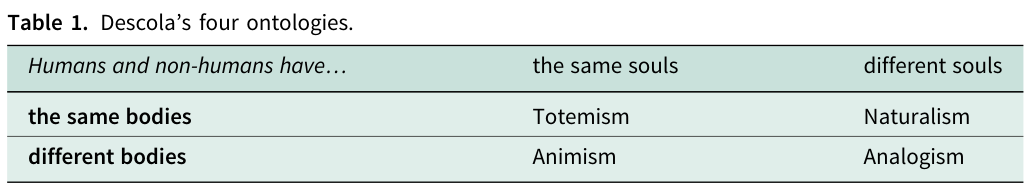
\includegraphics[width=\linewidth]{table1.png}\par
{\small Table 1, reproduced from the publisher PDF, p. 18.\par}\end{minipage}\end{center}
{\scriptsize\color{gray} [p. 18]}\ Joel Robbins’ work on moral torment and value conflict amongst Urapmin Christians (Robbins 2004) exemplifies this broad family of formalisms in a very different way. Robbins’ distinction between lawfulness and willfulness harks back explicitly to a Dumontian structuralist vision of pairs of values defined and tensed against each other (Robbins 2013b; 2015). The fact that there are two key values in play, which are logically opposed (like equality and hierarchy are for Dumont), is not a contingent but an essential part of the architecture of Robbins’s argument. Since for Robbins, as for Dumont, values are first and foremost \textit{relations}, their mathematics are grounded in powers of two. While Robbins does not go in for crossed tables, much of the rich complexity and elegance of his account of Urapmin moral life comes from the intersection between two relational pairs: a pair of values (willfulness—lawfulness) and a pair of contexts (traditional and Christian visions of the good).\par
{\scriptsize\color{gray} [p. 18]}\ This is not to say that the opposition between lawfulness and willfulness is merely a formal device, a conceptual system imposed from on high by the anthropologist. Lawfulness and willfulness (and indeed Christian and traditional) are paired opposites for the Urapmin themselves. As with the brotherhood/cousinage pair in Ben-Yehoyada’s case, contrastive pairing is also a pragmatic device that enables Urapmin to negotiate and understand their moral world. This is what we mean when we speak of an \textit{interface} between conceptual formalism and forms in the world: somewhere between the logical oppositions of interlocutors and those of the anthropologist, a systematic account arises. In this type of systematic formalism, ethnography and deductive logic work hand in hand to build such interfaces (Descola 2005b).\par
{\scriptsize\color{gray} [p. 18]}\ It is worth noting, however, that building systems out of logical contrasts is not the only topology of enclosure—not the only type of “sieve”—available to the new formalism. A different topology emerges from the formalist technique of building empirical lists that one could imagine extending or completing. It is enumerative rather than systematic (e.g., Luhrmann 2023). Staying with the theme of values, one might consider in this connection a recent article by Ori Mautner about value conflicts experienced by orthodox Israeli Jews engaging in collective mindfulness meditation (2025). In managing the tensions between traditional commitments and new practices, Mautner describes his interlocutors navigating between three different values: religious propriety (maintaining “traditionally sanctioned Jewish conduct and views”), spirituality (“developing self-acquaintance and consequently an increased intimacy with God”), and worldliness (“striving to sanctify rather than escape mundane life”). Unlike the contrast between lawfulness and willfulness, there is no inherent relationship or logical tension between these values, even though they may come into conflict in particular situations. Nor do they form a system that is coextensive with the nature of the problem at hand: one might imagine augmenting the account with other values—commitments to kin, perhaps. By contrast, to add a fifth ontology to Descola’s Big Four, or a third value to Robbins’s willfulness and lawfulness, one would need to recalibrate the entire system of their arguments.\par
{\scriptsize\color{gray} [p. 19]}\ This second type of formalist technique—building lists—is particularly clear in the recent interest in “modes,” sharply articulated by Michael Degani (2024). Drawing on examples ranging from post-socialist dance to paved road networks, he shows how anthropologists describe actors moving between different formalized patterns or styles, whether these are, for instance, bodily techniques, infrastructural systems, or ethical orientations. A Guinean dancer shifts between traditional and improvisational modes (Cohen 2016); a road system and dirt footpaths in New Guinea produce distinct forms of spiritual modality and gendered embodiment (Handman 2017); each mode has its constraints and affordances, but actors can often shift between them while maintaining their distinctiveness. Degani’s own work on modal reasoning and electrical infrastructure in Tanzania is itself a testament to the productive potential of “modality” as an anthropological form (2022; and see Kockelman 2020).\par
{\scriptsize\color{gray} [p. 19]}\ These two techniques of formalist conceptual enclosure—contrastive systems and open-ended lists—are not mutually exclusive: they can be deployed together and tensed against each other in the same accounts, to great effect. In Mautner’s argument, for instance, the potentially open-ended list of values is complemented by another distinction, this time a logical opposition, between “inherent” and “contingent” value conflicts. This distinction—which partly recoups our own distinction between two formalist techniques—itself takes the form of a logical opposition: value conflicts can be either inherent or they can be contingent. Forms of conceptual enclosure are not metaphysical commitments about the world (is it binary, systematic, open-ended?), nor do they need to be the battle-standards of opposing theoretical schools. Dichotomies, systems, typologies, and lists are, more simply and modestly, just tools—there to be used and recombined to solve particular empirical and conceptual problems.\par
\Needspace{5\baselineskip}\section*{The Epistemic Virtues of Formalism: Coherence, Corrigibility, Collaboration}
{\scriptsize\color{gray} [p. 19]}\ In contrasting lists and structures, we are not suggesting that these are the only two pathways to form. Quite the opposite, in fact: the new formalist sensibility we are mapping is distinguished precisely by its openness to the multiplicity and diversity of forms—both in the world and in our accounts of it. In this it differs sharply from the antiformalist intuition that form is one (bad) thing, and that it only warrants a single attitude (one of resistance or refusal).\par
{\scriptsize\color{gray} [p. 20]}\ Just as the new formalist sensibility doesn’t require a commitment to detailed ontological postulates about the nature of the world, so there is no single new formalist method, no rulebook or set of precise injunctions for how anthropological analysis must (or must not) be done. The examples we have described here differ in topic, tone, and theoretical orientation. The shift in sensibilities they share and exemplify is broader and more profound: rather than a precise program, it involves a growing affinity for certain epistemic virtues. The appeal to epistemic virtue is not new in anthropology. Antiformalism too had its own epistemic virtues built in. Revocability, flexibility, open-endedness, and the like were, in the antiformalist sensibility, the mark of the good in both scholarship and practical worldly activity, even as the formalist undercurrents and implications we have highlighted here persisted. The new formalism we describe here makes those implications and their associated virtues explicit, in an instance of Marilyn Strathern’s point that epochal change is often marked not by new practices but by new attitudes to practices that have always existed. We spotlight three formalist epistemic virtues that we feel are particularly characteristic of the current new moment: coherence, corrigibility, and collaboration.\par
{\scriptsize\color{gray} [p. 20]}\ New formalist work in anthropology tends toward the production of a coherent set of conceptual forms within a particular account. While acknowledging that the demand for coherence can be a power-laden imposition (Davé 2023), it nevertheless values self-imposed coherence in conceptual and analytical work: distinctions, categories, terminologies that sit in some stable relation to one another, concepts and terms that mean roughly the same thing from one page to the next. This commitment to one’s own coherence is also a commitment to a certain kind of accountability to others. Conceptual infrastructures, in this aesthetic, should come with “the possibility of (virtuous) failure” (Corsín Jiménez 2014: 385). If an account cannot be wrong, it has little value as an account of something outside itself, and little to add to a collective conversation. Fallibility and corrigibility are taken as key productive limitations in formalist accounts.\par
{\scriptsize\color{gray} [p. 20]}\ But corrigibility is not all about coherence. The new anthropological formalism comes with a commitment to some kind of strong relationship between conceptual forms and forms outside of the account. This relationship is often (whether anthropologists like to advertise this fact or not) one of classic representationalist correspondence. On some level, even the most conceptually sophisticated anthropological critics of old-fashioned realism still mostly write under the basic assumption that what they say is—broadly speaking—true to their ethnography. We have seen that this same spirit of realism in some ways underlies the aesthetic of emergence and process—that a world without form must be described by similarly “formless” accounts (as if such a thing were possible). And in its own way, the anti-representationalist vision of anthropological writing as performative engagement—writing as politics, “ontological” (Mol 2002) or otherwise—can be just as productively limiting. If conceptual forms are seen not as descriptions but as tools that enable an effective transformation of something beyond the account, then the limitation on what can be said is, if anything, even more stringent. For such performative conceptual forms need, after all, to work. Alongside a commitment to fallibility and to corrigibility, then, we might think of this second productive limitation not merely as “correspondence,” but as something broader—a kind of “worldliness.”\par
{\scriptsize\color{gray} [p. 21]}\ A third, and perhaps, most crucial form of productive limitation is an openness to disciplinary dialogue and crosswise critical engagement. As Boyer and Howe point out in a powerful reconceptualization of what anthropologists mean by “theory,” intradisciplinary dialogue—in the form of paper-giving, Q\&As, peer review, research supervision, collaborative writing, and the like—is fundamentally structured by an expectation that knowledge should travel. An anthropological account is expected to mobilize insights that become available to other accounts, to be “\textit{transparticular}, a study that speaks with other studies … to create the communicative pathways … that help to cohere anthropology as a distinctive field of discourse” (Boyer and Howe 2015). Transparticularity need not imply universality—few anthropologists today would promote the impractical vision of a grand unified anthropological discourse modeled on the “hard sciences.” Transparticularity is rather a matter of “portable analytics” (ibid.)—conceptual forms that travel from one account to another and can be repurposed or revised and passed on again.\par
{\scriptsize\color{gray} [p. 21]}\ As Boyer and Howe point out, anthropological accounts that do not acknowledge relevant previous attempts to grapple with similar problems tend to be dismissed as ungenerous. In recent years, this question has mostly been debated from the perspective of “input”: the—ethical and political as much as epistemic—question of how present accounts should build on previous ones and acknowledge what they “take.” This opens up a wide field of controversy over which previous accounts should be deemed relevant, rife with disputes over citational politics, epistemic justice, and the shape of the canon (Allen and Jobson 2016; Venkatesan 2025). The anthropological return to form, however, pays at least equal attention to the question of \textit{output}: what “portable analytics” is each account producing or refashioning for others to pick up? This means attending to transparticularity and collaboration not just as a question of how we ethically take from each other, but also as a question of how best to give.\par
{\scriptsize\color{gray} [p. 21]}\ In this connection, transparticularity/collaboration as an epistemic virtue rejoins corrigibility/worldliness. Concepts designed to be shared have to be carefully crafted to stand the test of other users––both in their internal architecture and in their external relation to the phenomena they purport to illuminate. Paradoxically, the antiformalist attitude has led to a proliferation of turns, neologisms, and conceptual distinctions, precisely because it eschewed the thought that these concepts might become stable tokens of collaboration. Coining new concepts, like passing new laws, is more immediately appealing than trying to apply the ones we already have. If concepts are just necessary evils on the path to an account of irreducible complexity, then there is little mileage in paying much attention to how they are crafted or in keeping them around after their work is done. Each individual account can provide its own conceptual revolution, and move on. The new formalist aesthetic, by contrast, keeps an eye on the pragmatics of conceptual reuse. Good tools are worth sharpening and fixing—one can lend and borrow them, too.\par
\Needspace{5\baselineskip}\section*{Conclusion: What Comes Next?}
{\scriptsize\color{gray} [p. 21]}\ The two ingredients of what we are calling a new formalist sensibility, then, are an attention to and puzzling over regularities in the world, and a commitment to crafting conceptual enclosures around them. These are not independent moves: regularities in the world often only become visible as they meet with our conceptual formalisms. Like (other) scientific objects, modes, values, cultures, trends, roles, techniques, kinship structures, and so forth are hybrids: they are the result of a successful articulation between a conceptual device and something in the world that “objects” back (Stengers 2000). Anthropological formalism as we conceive it requires some interface between conceptual forms and worldly regularities. This is not just a matter of “giving ethnographic phenomena particular conceptual shapes” (Holbraad 2020), but also of allowing the shape of phenomena to distort, guide, and object to the shape of our conceptual formalisms. Form—as Kingston (2003) observed in an early and profound call for a return to form in anthropology—is inherently related to attention: “Form itself only exists in relation to the formless, as areas of focused attention are relative to inattentiveness” (ibid.: 685). Conceptual formalisms, at their best, manifest a renewed commitment to a particular kind of attentiveness.\par
{\scriptsize\color{gray} [p. 22]}\ Yet this attention should extend also to the form/antiform dynamic as a whole. Insofar as a formalist aesthetic feels like it has momentum in contemporary anthropology, this momentum comes in part from pushing off from an older antiformalist consensus—form can only exist in relation to the formless. This is not in itself something to be either celebrated or regretted—it is the way of disciplinary enthusiasms, to get their drive from opposition. It simply reminds those who—like us—are enthused by the new formalist aesthetic that we may do well to keep asking what antiformalisms we still nevertheless value and deploy, and what is worth retaining from the antiformalist anthropological moment that is rapidly coming to feel historical.\par
{\scriptsize\color{gray} [p. 22]}\ The antiformalist aesthetic we began by describing served anthropology in innumerable ways, not least by helping first to dismantle and then to guard against the return of overly rigid structural models that threatened to flatten ethnographic complexity. This, though, is a different historical moment, and the threats the discipline (and the world) face are different too. Large language models have sparked public interest and debate about pattern recognition and the wider relationship between form and meaning. Political mobilizations of various types demand recognition of some stable categorical identities whilst insisting on the dissolution of others. Economic and professional life in Euro-America is increasingly suffused by concerns about managerialism, bureaucracy, and accountability. Meanwhile, as we have noted, popular discourse has seen the increasing deployment of antiformalist rhetoric in celebration of disruption and the rejection of expertise and institutional constraints, but toward ends that make antiformalism’s once clearly progressive gestures look newly concerning.\par
{\scriptsize\color{gray} [p. 22]}\ So the new formalist aesthetic we have sought to identify does not emerge from a nostalgia for past certainties, but from a belief in anthropology’s capacity to craft theories, arguments, and models that say something distinctive about the contemporary world’s complexity. Formal and anti-formal moves will continue to intertwine in anthropological work, and that oscillation is baked into the nature of the discipline. But there is more to such oscillation than mere intellectual fads or trends. Theoretical schools and turns might come and go, but the rise of form today, like that of practice in the 1980s, points to something more epochal and addresses fundamental intellectual and worldly challenges.\par
\Needspace{5\baselineskip}\section*{Acknowledgements}
{\scriptsize\color{gray} [p. 22]}\ The authors would like to thank Naor Ben-Yehoyada, Joanna Cook, Mike Degani, James Laidlaw, Adam Reed, Andrew Shryock, Marilyn Strathern, and Tom Yarrow for their very thoughtful views on earlier drafts of this paper. We are also grateful to Jatin Dua, Lauren Kapsalakis, and to four anonymous reviewers for their generous help in revising the paper for publication in CSSH.\par
\Needspace{5\baselineskip}\section*{References}
\noindent\begin{minipage}[t]{\linewidth}{\scriptsize\color{gray} [p. 23]}\ Agha, A. 2006. Language and Social Relations. Leiden: Cambridge University Press. At: \url{http://public.eblib.com/choice/publicfullrecord.aspx?p=279321,} accessed 21 December 2016. DOI: \url{10.1017/CBO9780511618284}\par\end{minipage}\par
\noindent\begin{minipage}[t]{\linewidth}{\scriptsize\color{gray} [p. 23]}\ Albris, K., Candea, M., Enggard, T., Jakobsen, T., and Pedersen, M.. 2025. Measuring MAN (incorporating JRAI): Computational Anthropological Analysis and Quantitative Speculation. Journal of the Royal Anthropological Institute 32 (July): 32–54. DOI: \url{10.1111/1467-9655.14290}\par\end{minipage}\par
\noindent\begin{minipage}[t]{\linewidth}{\scriptsize\color{gray} [p. 23]}\ Alexander, C. 2017. The Meeting as Subjunctive Form: Public/Private IT Projects in British and Turkish State Bureaucracies. Journal of the Royal Anthropological Institute 23, S1: 80–94. DOI: \url{10.1111/1467-9655.12595}\par\end{minipage}\par
\noindent\begin{minipage}[t]{\linewidth}{\scriptsize\color{gray} [p. 23]}\ Allen, J. S. and Jobson, R. C. 2016. The Decolonizing Generation: (Race and) Theory in Anthropology Since the Eighties. Current Anthropology 57, 2: 129–148. DOI: \url{10.1086/685502}\par\end{minipage}\par
\noindent\begin{minipage}[t]{\linewidth}{\scriptsize\color{gray} [p. 23]}\ Asad, T. 2003. Formations of the Secular: Christianity, Islam, Modernity. Stanford: Stanford University Press.\par\end{minipage}\par
\noindent\begin{minipage}[t]{\linewidth}{\scriptsize\color{gray} [p. 23]}\ Bandak, A. 2015. Exemplary Series and Christian Typology: Modelling on Sainthood in Damascus. Journal of the Royal Anthropological Institute. 21, S1: 47–63. DOI: \url{10.1111/1467-9655.12165}\par\end{minipage}\par
\noindent\begin{minipage}[t]{\linewidth}{\scriptsize\color{gray} [p. 23]}\ Barad, K. M. 2007. Meeting the Universe Halfway: Quantum Physics and the Entanglement of Matter and Meaning. Durham: Duke University Press. DOI: \url{10.2307/j.ctv12101zq}\par\end{minipage}\par
\noindent\begin{minipage}[t]{\linewidth}{\scriptsize\color{gray} [p. 23]}\ Bear, L., Ho, K., Tsing, A. L., and Yanagisako., S. 2015. Gens: A Feminist Manifesto for the Study of Capitalism. Society for Cultural Anthropology. \url{https://culanth.org.}\par\end{minipage}\par
\noindent\begin{minipage}[t]{\linewidth}{\scriptsize\color{gray} [p. 23]}\ Ben-Yehoyada, N. 2014. Transnational Political Cosmology: A Central Mediterranean Example. Comparative Studies in Society and History 56, 4: 870–901. DOI: \url{10.1017/S0010417514000437}\par\end{minipage}\par
\noindent\begin{minipage}[t]{\linewidth}{\scriptsize\color{gray} [p. 23]}\ Biehl, J. and Locke, P.. 2010. Deleuze and the Anthropology of Becoming. Current Anthropology 51, 3: 317–51. DOI: \url{10.1086/651466}\par\end{minipage}\par
\noindent\begin{minipage}[t]{\linewidth}{\scriptsize\color{gray} [p. 23]}\ Boellstorff, T. 2010. A Typology of Ethnographic Scales for Virtual Worlds. In Bainbridge, W. S., ed., Online Worlds: Convergence of the Real and the Virtual. London: Springer London, 123–33. DOI: \url{10.1007/978-1-84882-825-4_10}\par\end{minipage}\par
\noindent\begin{minipage}[t]{\linewidth}{\scriptsize\color{gray} [p. 23]}\ Bourdieu, P. 1977. Outline of a Theory of Practice. Cambridge: Cambridge University Press. DOI: \url{10.1017/CBO9780511812507}\par\end{minipage}\par
\noindent\begin{minipage}[t]{\linewidth}{\scriptsize\color{gray} [p. 23]}\ Boyer, D. 2013. Simply the Best: Parody and Political Sincerity in Iceland. American Ethnologist. 40, 2: 276–87. DOI: \url{10.1111/amet.12020}\par\end{minipage}\par
\noindent\begin{minipage}[t]{\linewidth}{\scriptsize\color{gray} [p. 23]}\ Boyer, D. and Howe, C.. 2015. Portable Analytics and Lateral Theory. In Boyer, D., Faubion, J., and Marcus, G., eds., Theory Can Be More than It Used to Be: Learning Anthropology’s Method in a Time of Transition. Ithaca: Cornell University Press, 15–38.\par\end{minipage}\par
\noindent\begin{minipage}[t]{\linewidth}{\scriptsize\color{gray} [p. 23]}\ Boyer, D. and Yurchak, A.. 2010. American Stiob: Or, What Late-Socialist Aesthetics of Parody Reveal about Contemporary Political Culture in the West. Cultural Anthropology 25, 2: 179–221. DOI: \url{10.1111/j.1548-1360.2010.01056.x}\par\end{minipage}\par
\noindent\begin{minipage}[t]{\linewidth}{\scriptsize\color{gray} [p. 23]}\ Bunzl, M. 2008. The Quest for Anthropological Relevance: Borgesian Maps and Epistemological Pitfalls. American Anthropologist 110, 1: 53–60. DOI: \url{10.1111/j.1548-1433.2008.00008.x}\par\end{minipage}\par
\noindent\begin{minipage}[t]{\linewidth}{\scriptsize\color{gray} [p. 23]}\ Candea, M. 2007. Arbitrary Locations: In Defence of the Bounded Field-Site. Journal of the Royal Anthropological Institute 13, 1: 167–84. DOI: \url{10.1111/j.1467-9655.2007.00419.x}\par\end{minipage}\par
\noindent\begin{minipage}[t]{\linewidth}{\scriptsize\color{gray} [p. 23]}\ Candea, M. 2016. We Have Never Been Pluralist: On Lateral and Frontal Comparisons in the Ontological Turn. In Charbonnier, P., Salmon, G., and Skafish, P., eds., Comparative Metaphysics: Ontology after Anthropology. London: Rowman \& Littlefield, 85–106. DOI: \url{10.5040/9798881812645.ch-4}\par\end{minipage}\par
\noindent\begin{minipage}[t]{\linewidth}{\scriptsize\color{gray} [p. 23]}\ Candea, M. 2019. Comparison in Anthropology: The Impossible Method. Cambridge: Cambridge University Press.\par\end{minipage}\par
\noindent\begin{minipage}[t]{\linewidth}{\scriptsize\color{gray} [p. 23]}\ Candea, M. 2025. A Return to Form. Social Analysis 69, 1. DOI: \url{10.3167/sa.2025.690103}\par\end{minipage}\par
\noindent\begin{minipage}[t]{\linewidth}{\scriptsize\color{gray} [p. 23]}\ Clarke, M. 2015. Legalism and the Care of the Self: Sharīʿah Discourse in Contemporary Lebanon. In Dresch, P. and Scheele, J., eds., Legalism: Rules and Categories. Oxford Scholarship Online, 231–57. DOI: \url{10.1093/acprof:oso/9780198753810.003.0010}\par\end{minipage}\par
\noindent\begin{minipage}[t]{\linewidth}{\scriptsize\color{gray} [p. 23]}\ Clifford, J. 1981. On Ethnographic Surrealism. Comparative Studies in Society and History 23, 4: 539–64. DOI: \url{10.1017/S0010417500013554}\par\end{minipage}\par
\noindent\begin{minipage}[t]{\linewidth}{\scriptsize\color{gray} [p. 23]}\ Cohen, A. 2016. Inalienable Performances, Mutable Heirlooms: Dance, Cultural Inheritance, and Political Transformation in the Republic of Guinea. American Ethnologist 43, 4: 650–62. DOI: \url{10.1111/amet.12381}\par\end{minipage}\par
\noindent\begin{minipage}[t]{\linewidth}{\scriptsize\color{gray} [p. 23]}\ Coole, D. and Frost, S.. 2010. New Materialisms: Ontology, Agency, and Politics. Durham: Duke University Press.\par\end{minipage}\par
\noindent\begin{minipage}[t]{\linewidth}{\scriptsize\color{gray} [p. 23]}\ Corsín Jiménez, A. 2014. Introduction: The Prototype: More than Many and Less than One. Journal of Cultural Economy. 7, 4: 381–98. DOI: \url{10.1080/17530350.2013.858059}\par\end{minipage}\par
\noindent\begin{minipage}[t]{\linewidth}{\scriptsize\color{gray} [p. 23]}\ Culler, J. 2018. 1980: Structuralism and Poststructuralism. Ex-position 40: 79–94.\par\end{minipage}\par
\noindent\begin{minipage}[t]{\linewidth}{\scriptsize\color{gray} [p. 24]}\ Davé, N. N. 2023. Indifference: On the Praxis of Interspecies Being. Duke University Press Books.\par\end{minipage}\par
\noindent\begin{minipage}[t]{\linewidth}{\scriptsize\color{gray} [p. 24]}\ Degani, M. 2022. The City Electric: Infrastructure and Ingenuity in Postsocialist Tanzania. Durham: Duke University Press.\par\end{minipage}\par
\noindent\begin{minipage}[t]{\linewidth}{\scriptsize\color{gray} [p. 24]}\ Degani, M. 2024. Toward a Modal Anthropology. Social Analysis. 68, 3: 60–84. DOI: \url{10.3167/sa.2024.680304}\par\end{minipage}\par
\noindent\begin{minipage}[t]{\linewidth}{\scriptsize\color{gray} [p. 24]}\ Deleuze, G. 1997. Essays Critical and Clinical. Minneapolis: University of Minnesota Press.\par\end{minipage}\par
\noindent\begin{minipage}[t]{\linewidth}{\scriptsize\color{gray} [p. 24]}\ Deleuze, G. and Guattari, F.. 1988. Capitalism and Schizophrenia II: A Thousand Plateaus. London: The Athlone Press.\par\end{minipage}\par
\noindent\begin{minipage}[t]{\linewidth}{\scriptsize\color{gray} [p. 24]}\ Deluermoz, Q. and Singaravélou, P.. 2016. Pour une Histoire des Possibles: Analyses Contrefactuelles et Futurs Non Advenus. Paris: Editions Seuil.\par\end{minipage}\par
\noindent\begin{minipage}[t]{\linewidth}{\scriptsize\color{gray} [p. 24]}\ Descola, P. 2005a. Par Delà Nature et Culture. Paris: Gallimard.\par\end{minipage}\par
\noindent\begin{minipage}[t]{\linewidth}{\scriptsize\color{gray} [p. 24]}\ Descola, P. 2005b. On Anthropological Knowledge. Social Anthropology. 13, 1: 65–73. DOI: \url{10.1017/S0964028204000849}\par\end{minipage}\par
\noindent\begin{minipage}[t]{\linewidth}{\scriptsize\color{gray} [p. 24]}\ Dresch, P. 1986. The Significance of the Course Events Take in Segmentary Systems. American Ethnologist 13, 2: 309–24. DOI: \url{10.1525/ae.1986.13.2.02a00070}\par\end{minipage}\par
\noindent\begin{minipage}[t]{\linewidth}{\scriptsize\color{gray} [p. 24]}\ Dresch, P. 1998. Mutual Deception. Totality, Exchange, and Islam in the Middle East. In James, W. and Allen, N. J., eds., Marcel Mauss: A Centenary Tribute. Oxford: Berghahn, 111–33. DOI: \url{10.2307/j.ctv287sjvt.12}\par\end{minipage}\par
\noindent\begin{minipage}[t]{\linewidth}{\scriptsize\color{gray} [p. 24]}\ Dua, J. 2019a. Hijacked: Piracy and Economies of Protection in the Western Indian Ocean. Comparative Studies in Society and History 61, 3: 479–507. DOI: \url{10.1017/S0010417519000215}\par\end{minipage}\par
\noindent\begin{minipage}[t]{\linewidth}{\scriptsize\color{gray} [p. 24]}\ Dua, J. 2019b. Captured at Sea: Piracy and Protection in the Indian Ocean. Berkeley: University of California Press. DOI: \url{10.2307/j.ctvp2n2sr}\par\end{minipage}\par
\noindent\begin{minipage}[t]{\linewidth}{\scriptsize\color{gray} [p. 24]}\ Du Gay, P. 2000. In Praise of Bureaucracy: Weber, Organization, Ethics. London, Thousand Oaks: SAGE. DOI: \url{10.4135/9781446217580}\par\end{minipage}\par
\noindent\begin{minipage}[t]{\linewidth}{\scriptsize\color{gray} [p. 24]}\ Edwards, J. 2000. Born and Bred: Idioms of Kinship and New Reproductive Technologies in England. London: Routledge. DOI: \url{10.1093/oso/9780198233947.001.0001}\par\end{minipage}\par
\noindent\begin{minipage}[t]{\linewidth}{\scriptsize\color{gray} [p. 24]}\ Faubion, J. D. 2011. An Anthropology of Ethics. New York: Cambridge University Press. DOI: \url{10.1017/CBO9780511792557}\par\end{minipage}\par
\noindent\begin{minipage}[t]{\linewidth}{\scriptsize\color{gray} [p. 24]}\ Fleming, L. 2024. On Speaking Terms: Avoidance Registers and the Sociolinguistics of Kinship. Toronto: University of Toronto Press. DOI: \url{10.3138/9781487550912}\par\end{minipage}\par
\noindent\begin{minipage}[t]{\linewidth}{\scriptsize\color{gray} [p. 24]}\ Gandolfo, D. 2013. FORMLESS: A Day at Lima’s Office of Formalization. Cultural Anthropology 28, 2: 278–98. DOI: \url{10.1111/cuan.12004}\par\end{minipage}\par
\noindent\begin{minipage}[t]{\linewidth}{\scriptsize\color{gray} [p. 24]}\ Garcia, T. 2018. The Life Intense: A Modern Obsession. Edinburgh: Edinburgh University Press. DOI: \url{10.3917/autre.garci.2018.01}\par\end{minipage}\par
\noindent\begin{minipage}[t]{\linewidth}{\scriptsize\color{gray} [p. 24]}\ Geertz, C., Geertz, H., and Rosen, L. 1979. Meaning and Order in Moroccan Society: Three Essays in Cultural Analysis. Cambridge: Cambridge University Press.\par\end{minipage}\par
\noindent\begin{minipage}[t]{\linewidth}{\scriptsize\color{gray} [p. 24]}\ Handelman, D., Shapiro, M., and Feldman, J.. 2020. Moebius Anthropology: Essays on the Forming of Form. Berghahn Books.\par\end{minipage}\par
\noindent\begin{minipage}[t]{\linewidth}{\scriptsize\color{gray} [p. 24]}\ Handman, C. 2017. Walking Like a Christian: Roads, Translation, and Gendered Bodies as Religious Infrastructure in Papua New Guinea. American Ethnologist 44: 315–27. DOI: \url{10.1111/amet.12481}\par\end{minipage}\par
\noindent\begin{minipage}[t]{\linewidth}{\scriptsize\color{gray} [p. 24]}\ Helmreich, S. 2014. Waves: An Anthropology of Scientific Things. HAU: Journal of Ethnographic Theory 4, 3: 265–84 DOI: \url{10.14318/hau4.3.016}\par\end{minipage}\par
\noindent\begin{minipage}[t]{\linewidth}{\scriptsize\color{gray} [p. 24]}\ Heywood, P. 2012. Anthropology and What There Is: Reflections on “Ontology.” The Cambridge Journal of Anthropology 30, 1: 143–51. DOI: \url{10.3167/ca.2012.300112}\par\end{minipage}\par
\noindent\begin{minipage}[t]{\linewidth}{\scriptsize\color{gray} [p. 24]}\ Heywood, P. 2023. Out of the Ordinary: Everyday Life and the Carnival of Mussolini. American Anthropologist 125, 3: 493–504. DOI: \url{10.1111/aman.13850}\par\end{minipage}\par
\noindent\begin{minipage}[t]{\linewidth}{\scriptsize\color{gray} [p. 24]}\ Heywood, P. 2024. Burying Mussolini: Ordinary Life in the Shadows of Fascism. Ithaca: Cornell University Press.\par\end{minipage}\par
\noindent\begin{minipage}[t]{\linewidth}{\scriptsize\color{gray} [p. 24]}\ Heywood, P. 2026. The Life of Form: Anthropology, Wittgenstein, and the Problem of Context. Cambridge: Cambridge University Press. DOI: \url{10.1017/9781009356626}\par\end{minipage}\par
\noindent\begin{minipage}[t]{\linewidth}{\scriptsize\color{gray} [p. 24]}\ Heywood, P. and Candea, M., eds. 2023. Beyond Description: Anthropologies of Explanation. Ithaca: Cornell University Press. DOI: \url{10.1515/9781501771583}\par\end{minipage}\par
\noindent\begin{minipage}[t]{\linewidth}{\scriptsize\color{gray} [p. 24]}\ Heywood, P. and Yarrow, T. 2026. On the Problem of Continuity: A Theory of Culture Beyond Invention. Journal of the Royal Anthropological Institute 32, 2\textit{:} 365–83. DOI: \url{10.1111/1467-9655.70023}\par\end{minipage}\par
\noindent\begin{minipage}[t]{\linewidth}{\scriptsize\color{gray} [p. 24]}\ Højer, L. and Bandak, A.. 2015. Introduction: The Power of Example. Journal of the Royal Anthropological Institute. 21, S1: 1–17. DOI: \url{10.1111/1467-9655.12173}\par\end{minipage}\par
\noindent\begin{minipage}[t]{\linewidth}{\scriptsize\color{gray} [p. 24]}\ Holbraad, M. 2020. The Shapes of Relations: Anthropology as Conceptual Morphology. Philosophy of the Social Sciences. 50, 6: 495–522. DOI: \url{10.1177/0048393120917917}\par\end{minipage}\par
\noindent\begin{minipage}[t]{\linewidth}{\scriptsize\color{gray} [p. 24]}\ Howe, C. and Boyer, D.. 2015. Portable Analytics and Lateral Theory. In Boyer, D., Faubion, J. D., and Marcus, G. E., eds., Theory Can Be More than It Used to Be: Learning Anthropology’s Method in a Time of Transition. Cornell University Press, 15–38.\par\end{minipage}\par
\noindent\begin{minipage}[t]{\linewidth}{\scriptsize\color{gray} [p. 24]}\ Hull, M. 2012. Documents and Bureaucracy. Annual Review of Anthropology 41: 251–67. DOI: \url{10.1146/annurev.anthro.012809.104953}\par\end{minipage}\par
\noindent\begin{minipage}[t]{\linewidth}{\scriptsize\color{gray} [p. 25]}\ Humphrey, C. 2008. Reassembling Individual Subjects: Events and Decisions in Troubled Times. Anthropological Theory 8, 4: 357–80. DOI: \url{10.1177/1463499608096644}\par\end{minipage}\par
\noindent\begin{minipage}[t]{\linewidth}{\scriptsize\color{gray} [p. 25]}\ Humphrey, C. 2020. Real Estate Speculation: Volatile Social Forms at a Global Frontier of Capital. Economy and Society 49: 116–40. DOI: \url{10.1080/03085147.2019.1690256}\par\end{minipage}\par
\noindent\begin{minipage}[t]{\linewidth}{\scriptsize\color{gray} [p. 25]}\ Humphrey, C. and Laidlaw, J.. 1994. The Archetypal Actions of Ritual: A Theory of Ritual Illustrated by the Jain Rite of Worship, Vol. Oxford Studies in Social and Cultural Anthropology. Oxford New York: Clarendon Press Oxford University Press. DOI: \url{10.1093/oso/9780198277880.001.0001}\par\end{minipage}\par
\noindent\begin{minipage}[t]{\linewidth}{\scriptsize\color{gray} [p. 25]}\ Jackson, S. 2013. Rethinking Repair: Media Meets Technology. Cambridge: MIT Press.\par\end{minipage}\par
\noindent\begin{minipage}[t]{\linewidth}{\scriptsize\color{gray} [p. 25]}\ Jobson, R. C. 2020. The Case for Letting Anthropology Burn: Sociocultural Anthropology in 2019. American Anthropologist 122, 2: 259–71. DOI: \url{10.1111/aman.13398}\par\end{minipage}\par
\noindent\begin{minipage}[t]{\linewidth}{\scriptsize\color{gray} [p. 25]}\ Kavedžija, I. 2018. Of Manners and Hedgehogs: Building Closeness by Maintaining Distance. The Australian Journal of Anthropology 29, 2: 146–157. At: \url{https://onlinelibrary.wiley.com/doi/abs/10.1111/taja.12274,} accessed 17 March 2021.\par\end{minipage}\par
\noindent\begin{minipage}[t]{\linewidth}{\scriptsize\color{gray} [p. 25]}\ Kavedžija, I. 2019. Making Meaningful Lives: Tales from an Aging Japan. Contemporary Ethnography Series. University of Pennsylvania Press.\par\end{minipage}\par
\noindent\begin{minipage}[t]{\linewidth}{\scriptsize\color{gray} [p. 25]}\ Keane, W. 1997. Signs of Recognition: Powers and Hazards of Representation in an Indonesian Society. University of California Press. DOI: \url{10.1525/9780520917637}\par\end{minipage}\par
\noindent\begin{minipage}[t]{\linewidth}{\scriptsize\color{gray} [p. 25]}\ Keane, W. 2018. On Semiotic Ideology. Signs and Society 6, 1: 1–24. DOI: \url{10.1086/695387}\par\end{minipage}\par
\noindent\begin{minipage}[t]{\linewidth}{\scriptsize\color{gray} [p. 25]}\ Kelty, C. M. 2016. Too Much Democracy in All the Wrong Places: Toward a Grammar of Participation. Current Anthropology 58, S15: S77–90. DOI: \url{10.1086/688705}\par\end{minipage}\par
\noindent\begin{minipage}[t]{\linewidth}{\scriptsize\color{gray} [p. 25]}\ Kingston, S. 2003. Form, Attention and a Southern New Ireland life Cycle. Journal of the Royal Anthropological Institute 9, 4: 681–708. DOI: \url{10.1111/j.1467-9655.2003.00169.x}\par\end{minipage}\par
\noindent\begin{minipage}[t]{\linewidth}{\scriptsize\color{gray} [p. 25]}\ Kockelman, P. 2013. The Anthropology of an Equation: Sieves, Spam Filters, Agentive Algorithms, and Ontologies of Transformation. Hau: Journal of Ethnographic Theory 3, 3: 33–61. DOI: \url{10.14318/hau3.3.003}\par\end{minipage}\par
\noindent\begin{minipage}[t]{\linewidth}{\scriptsize\color{gray} [p. 25]}\ Kockelman, P. 2020. Kinds of Value: An Experiment in Modal Anthropology. Chicago: University of Chicago Press.\par\end{minipage}\par
\noindent\begin{minipage}[t]{\linewidth}{\scriptsize\color{gray} [p. 25]}\ Krøijer, S. 2015. Figurations of the Future: Forms and Temporalities of Left Radical Politics in Northern Europe. London: Berghahn Books.\par\end{minipage}\par
\noindent\begin{minipage}[t]{\linewidth}{\scriptsize\color{gray} [p. 25]}\ Laidlaw, J. 1995. Riches and Renunciation. Oxford: Clarendon Press. DOI: \url{10.1093/oso/9780198280316.001.0001}\par\end{minipage}\par
\noindent\begin{minipage}[t]{\linewidth}{\scriptsize\color{gray} [p. 25]}\ Laidlaw, J. and Heywood, P.. 2013. One More Turn and You’re There. Anthropology of this Century 7.\par\end{minipage}\par
\noindent\begin{minipage}[t]{\linewidth}{\scriptsize\color{gray} [p. 25]}\ Langlitz, N. 2020. Devil’s Advocate: Sketch of an Amoral Anthropology. HAU: Journal of Ethnographic Theory 10, 3: 989–1004. DOI: \url{10.1086/711682}\par\end{minipage}\par
\noindent\begin{minipage}[t]{\linewidth}{\scriptsize\color{gray} [p. 25]}\ Larkin, B. 2017. Promising Forms. The Political Aesthetics of Infrastructure. In Anand, N., Gupta, A. F., and Appel, H., eds., The Promise of Infrastructure. Durham: Duke University Press, 175\textit{–} 202.\par\end{minipage}\par
\noindent\begin{minipage}[t]{\linewidth}{\scriptsize\color{gray} [p. 25]}\ Latour, B. 2005. Reassembling the Social: An Introduction to Actor-Network-Theory. Oxford: Oxford University Press. DOI: \url{10.1093/oso/9780199256044.001.0001}\par\end{minipage}\par
\noindent\begin{minipage}[t]{\linewidth}{\scriptsize\color{gray} [p. 25]}\ Leach, J. 2015. The Death of a Drum: Objects, Persons, and Changing Social Form on the Rai Coast of Papua New Guinea. Journal of the Royal Anthropological Institute 21, 3: 620–40. DOI: \url{10.1111/1467-9655.12253}\par\end{minipage}\par
\noindent\begin{minipage}[t]{\linewidth}{\scriptsize\color{gray} [p. 25]}\ Lempert, M. 2012. Discipline and Debate: The Language of Violence in a Tibetan Buddhist Monastery. Berkeley: University of California Press.\par\end{minipage}\par
\noindent\begin{minipage}[t]{\linewidth}{\scriptsize\color{gray} [p. 25]}\ Lempert, M. 2025. From Small Talk to Microaggression: A History of Scale. Chicago: University of Chicago Press.\par\end{minipage}\par
\noindent\begin{minipage}[t]{\linewidth}{\scriptsize\color{gray} [p. 25]}\ Limbert, M. 2025. Homeland Is Where the Soul Rises: Travel Prayer, Passports, and Nation in the Western Indian Ocean. Comparative Studies in Society and History 67, 2: 457–82. DOI: \url{10.1017/S0010417524000409}\par\end{minipage}\par
\noindent\begin{minipage}[t]{\linewidth}{\scriptsize\color{gray} [p. 25]}\ Lord Smail, D. and Shryock, A.. 2013. History and the “Pre.” American Historical Review 118, 3: 709–37. DOI: \url{10.1093/ahr/118.3.709}\par\end{minipage}\par
\noindent\begin{minipage}[t]{\linewidth}{\scriptsize\color{gray} [p. 25]}\ Luhrmann, T. 2023. On Anthropological Findings. In Heywood, P. and Candea, M., eds., Beyond Description: Anthropologies of Explanation. Cornell: Cornell University Press, 45–62. DOI: \url{10.1515/9781501771583-004}\par\end{minipage}\par
\noindent\begin{minipage}[t]{\linewidth}{\scriptsize\color{gray} [p. 25]}\ Marcus, G. E. 2007. Ethnography Two Decades after Writing Culture: From the Experimental to the Baroque. Anthropological Quarterly 80, 4: 1127–45. DOI: \url{10.1353/anq.2007.0059}\par\end{minipage}\par
\noindent\begin{minipage}[t]{\linewidth}{\scriptsize\color{gray} [p. 25]}\ Martin, E. 1994. Flexible Bodies: Tracking Immunity in American Culture from the Days of Polio to the Age of AIDS. Boston: Beacon Press.\par\end{minipage}\par
\noindent\begin{minipage}[t]{\linewidth}{\scriptsize\color{gray} [p. 25]}\ Maurer, B. 2012. Payment: Forms and Functions of Value Transfer in Contemporary Society. The Cambridge Journal of Anthropology. 30, 2: 15–35. DOI: \url{10.3167/ca.2012.300202}\par\end{minipage}\par
\noindent\begin{minipage}[t]{\linewidth}{\scriptsize\color{gray} [p. 25]}\ Mautner, O. 2025. Struggling to Uplift Divine Sparks: Implicit Strategies for Handling Value Conflicts among Orthodox Jewish Meditators and Beyond. Current Anthropology 66, 6: 837–862. DOI: \url{10.1086/738531}\par\end{minipage}\par
\noindent\begin{minipage}[t]{\linewidth}{\scriptsize\color{gray} [p. 26]}\ Mcgranahan, C. 2016. Theorizing Refusal: An Introduction. Cultural Anthropology 31, 3: 319–325. DOI: \url{10.14506/ca31.3.01}\par\end{minipage}\par
\noindent\begin{minipage}[t]{\linewidth}{\scriptsize\color{gray} [p. 26]}\ McKinnon, S. and Cannell, F., eds. 2015. Vital Relations: Modernity and the Persistent Life of Kinship. School for Advanced Research Press. First edition.\par\end{minipage}\par
\noindent\begin{minipage}[t]{\linewidth}{\scriptsize\color{gray} [p. 26]}\ Miyazaki, H. 2004. The Method of Hope: Anthropology, Philosophy, and Fijian Knowledge. Stanford: Stanford University Press. DOI: \url{10.1515/9781503624429}\par\end{minipage}\par
\noindent\begin{minipage}[t]{\linewidth}{\scriptsize\color{gray} [p. 26]}\ Mol, A. 2002. The Body Multiple: Ontology in Medical Practice. Durham: Duke University Press. DOI: \url{10.1215/9780822384151}\par\end{minipage}\par
\noindent\begin{minipage}[t]{\linewidth}{\scriptsize\color{gray} [p. 26]}\ Muehlebach, A. K. 2010. The Moral Neoliberal: Welfare and Citizenship in Italy. Chicago: University of Chicago Press.\par\end{minipage}\par
\noindent\begin{minipage}[t]{\linewidth}{\scriptsize\color{gray} [p. 26]}\ Ortner, S. B. 1984. Theory in Anthropology since the Sixties. Comparative Studies in Society and History. 26, 1: 126–66. DOI: \url{10.1017/S0010417500010811}\par\end{minipage}\par
\noindent\begin{minipage}[t]{\linewidth}{\scriptsize\color{gray} [p. 26]}\ Ortner, S. B. 2015. Dark Anthropology and Its Others: Theory since the Eighties. HAU: Journal of Ethnographic Theory 6, 1: 47–73. DOI: \url{10.14318/hau6.1.004}\par\end{minipage}\par
\noindent\begin{minipage}[t]{\linewidth}{\scriptsize\color{gray} [p. 26]}\ Rabinow, P. 1989. French Modern: Norms and Forms of the Social Environment. Cambridge: MIT Press.\par\end{minipage}\par
\noindent\begin{minipage}[t]{\linewidth}{\scriptsize\color{gray} [p. 26]}\ Rabinow, P. 1996. Ess\textit{ays on the Anthropology of Reason}. Princeton: Princeton University Press.\par\end{minipage}\par
\noindent\begin{minipage}[t]{\linewidth}{\scriptsize\color{gray} [p. 26]}\ Rees, T. 2018. After Ethnos. Durham: Duke University Press.\par\end{minipage}\par
\noindent\begin{minipage}[t]{\linewidth}{\scriptsize\color{gray} [p. 26]}\ Robbins, J. 2004. Becoming Sinners: Christianity and Moral Torment in a Papua New Guinea Society. Berkeley: University of California Press.\par\end{minipage}\par
\noindent\begin{minipage}[t]{\linewidth}{\scriptsize\color{gray} [p. 26]}\ Robbins, J. 2007. Continuity Thinking and the Problem of Christian Culture: Belief, Time, and the Anthropology of Christianity. Current Anthropology 48, 1: 5–38. DOI: \url{10.1086/508690}\par\end{minipage}\par
\noindent\begin{minipage}[t]{\linewidth}{\scriptsize\color{gray} [p. 26]}\ Robbins, J. 2013a. Beyond the Suffering Subject: Toward an Anthropology of the Good. Journal of the Royal Anthropological Institute 19, 3: 447–462. DOI: \url{10.1111/1467-9655.12044}\par\end{minipage}\par
\noindent\begin{minipage}[t]{\linewidth}{\scriptsize\color{gray} [p. 26]}\ Robbins, J. 2013b. Monism, Pluralism and the Structure of Value Relations: A Dumontian Contribution to the Contemporary Study of Value. HAU: Journal of Ethnographic Theory 3, 1: 99–115. DOI: \url{10.14318/hau3.1.008}\par\end{minipage}\par
\noindent\begin{minipage}[t]{\linewidth}{\scriptsize\color{gray} [p. 26]}\ Robbins, J. 2015. Dumont’s Hierarchical Dynamism: Christianity and Individualism Revisited. HAU: Journal of Ethnographic Theory 5, 1: 173–95. DOI: \url{10.14318/hau5.1.009}\par\end{minipage}\par
\noindent\begin{minipage}[t]{\linewidth}{\scriptsize\color{gray} [p. 26]}\ Sahlins, M. 2002. Waiting for Foucault, Still. Chicago: Prickly Paradigm Press.\par\end{minipage}\par
\noindent\begin{minipage}[t]{\linewidth}{\scriptsize\color{gray} [p. 26]}\ Sanchez, A. 2023. Kill Your Ancestors: The Wars of Decolonization. American Ethnologist 50, 3: 435–45. DOI: \url{10.1111/amet.13190}\par\end{minipage}\par
\noindent\begin{minipage}[t]{\linewidth}{\scriptsize\color{gray} [p. 26]}\ Sanchez, A. 2024. Why Do We Need the Gens Manifesto? \textit{BoasBlog.} At: \url{https://boasblogs.org/researchingcapitalism/epilogue-why-do-we-need-the-gens-manifesto/.}\par\end{minipage}\par
\noindent\begin{minipage}[t]{\linewidth}{\scriptsize\color{gray} [p. 26]}\ Scheele, J. and Shryock, A. 2019. The Scandal of Continuity in Middle East Anthropology: Form, Duration, Difference. Bloomington: Indiana University Press. DOI: \url{10.2307/j.ctvpmw50z}\par\end{minipage}\par
\noindent\begin{minipage}[t]{\linewidth}{\scriptsize\color{gray} [p. 26]}\ Shapiro, M. 2016. Curving the Social, or, Why Antagonistic Rituals in Brazil are Variations on a Theme. Journal of the Royal Anthropological Institute. 22, 1: 47–66. DOI: \url{10.1111/1467-9655.12333}\par\end{minipage}\par
\noindent\begin{minipage}[t]{\linewidth}{\scriptsize\color{gray} [p. 26]}\ Shryock, A. 1997. Nationalism and the Genealogical Imagination: Oral History and Textual Authority in Tribal Jordan. \textit{Comparative Studies on Muslim Societies}, Vol. 23. Berkeley: University of California Press. DOI: \url{10.1525/9780520916388}\par\end{minipage}\par
\noindent\begin{minipage}[t]{\linewidth}{\scriptsize\color{gray} [p. 26]}\ Shweder, R. 2007. The Resolute Irresolution of Clifford Geertz. Common Knowledge 13, 2–3: 191–205. DOI: \url{10.1215/0961754X-2007-001}\par\end{minipage}\par
\noindent\begin{minipage}[t]{\linewidth}{\scriptsize\color{gray} [p. 26]}\ Silverstein, M. 1976. Shifters, Linguistic Categories, and Cultural Description. In Basso, K. H. and Selby, H., eds., A Meaning in Anthropology. Albuquerque: University of New Mexico Press, 11–55.\par\end{minipage}\par
\noindent\begin{minipage}[t]{\linewidth}{\scriptsize\color{gray} [p. 26]}\ Simpson, A. 2016. Consent’s Revenge. Cultural Anthropology 31, 3: 326–333. DOI: \url{10.14506/ca31.3.02}\par\end{minipage}\par
\noindent\begin{minipage}[t]{\linewidth}{\scriptsize\color{gray} [p. 26]}\ Stasch, R. 2009. Society of Others: Kinship and Mourning in a West Papuan Place. Berkeley: University of California Press. DOI: \url{10.1525/9780520943322}\par\end{minipage}\par
\noindent\begin{minipage}[t]{\linewidth}{\scriptsize\color{gray} [p. 26]}\ Stengers, I. 2000. The Invention of Modern Science. Minneapolis: University of Minnesota Press.\par\end{minipage}\par
\noindent\begin{minipage}[t]{\linewidth}{\scriptsize\color{gray} [p. 26]}\ Strathern, M. 1987. Out of Context: The Persuasive Fictions of Anthropology [and Comments and Reply]. Current Anthropology. 28, 3: 251–81. DOI: \url{10.1086/203527}\par\end{minipage}\par
\noindent\begin{minipage}[t]{\linewidth}{\scriptsize\color{gray} [p. 26]}\ Strathern, M. 1988. The Gender of the Gift: Problems with Women and Problems with Society in Melanesia. London: University of California Press. DOI: \url{10.1525/california/9780520064232.001.0001}\par\end{minipage}\par
\noindent\begin{minipage}[t]{\linewidth}{\scriptsize\color{gray} [p. 26]}\ Strathern, M. 1992. After Nature: English Kinship in the Late 20th Century. Cambridge: Cambridge University Press.\par\end{minipage}\par
\noindent\begin{minipage}[t]{\linewidth}{\scriptsize\color{gray} [p. 26]}\ Summerson Carr, E. and Lempert, M.. 2016. Scale: Discourse and Dimensions of Social Life. Berkeley: University of California Press. DOI: \url{10.1525/luminos.15}\par\end{minipage}\par
\noindent\begin{minipage}[t]{\linewidth}{\scriptsize\color{gray} [p. 26]}\ Tsing, Anna 2000. The Global Situation. Cultural Anthropology 15, 3: 327–60. DOI: \url{10.1525/can.2000.15.3.327}\par\end{minipage}\par
\noindent\begin{minipage}[t]{\linewidth}{\scriptsize\color{gray} [p. 26]}\ Tsing, A. 2010. Worlding the Matsutake Diaspora, or, Can Actor-Network-Theory Experiment With Holism? In Otto, T., ed., Worlding the Matsutake Diaspora, or, Can Actor-Network-Theory Experiment with Holism? Vol. Experiments in Holism: Theory and Practice in Contemporary Anthropology. Oxford: Wiley-Blackwell, 47–66. DOI: \url{10.1002/9781444324426.ch4}\par\end{minipage}\par
\noindent\begin{minipage}[t]{\linewidth}{\scriptsize\color{gray} [p. 27]}\ Venkatesan, S. 2025. Decolonizing Anthropology: An Introduction. Polity Press.\par\end{minipage}\par
\noindent\begin{minipage}[t]{\linewidth}{\scriptsize\color{gray} [p. 27]}\ Woolard, K. A. and Schieffelin, B. B. 1994. Language Ideology. Annual Review of Anthropology 23: 55–82 At: \url{http://www.annualreviews.org/doi/pdf/10.1146/annurev.an.23.100194.000415,} accessed 24 January 2017.\par\end{minipage}\par
\noindent\begin{minipage}[t]{\linewidth}{\scriptsize\color{gray} [p. 27]}\ Yurchak, A. 2008. Necro-Utopia: The Politics of Indistinction and the Aesthetics of the Non-Soviet. Current Anthropology. 49, 2: 199–224. DOI: \url{10.1086/526098}\par\end{minipage}\par
\noindent\begin{minipage}[t]{\linewidth}{\scriptsize\color{gray} [p. 27]}\ Zuckerman, C. 2020. “Don’t Gamble for Money with Friends”: Moral-Economic Types and Their Uses. American Ethnologist 47, 4: 432–446. DOI: \url{10.1111/amet.12981}\par\end{minipage}\par
\end{document}
